% ============================================================
%  Radial-Cyclic Field Model — Full Paper Draft
%  Version 1.1 — Resolved-problems integration
%  Compile with: pdflatex rcfm.tex && bibtex rcfm &&
%                pdflatex rcfm.tex && pdflatex rcfm.tex
% ============================================================
\documentclass[10pt,twocolumn]{article}

% ── Packages ────────────────────────────────────────────────
\usepackage{amsmath,amssymb,amsfonts,amsthm}
\usepackage{cuted}
\usepackage[a4paper,margin=1.0in]{geometry}
\usepackage[colorlinks=true,
            linkcolor=blue!60!black,
            citecolor=blue!60!black,
            urlcolor=blue!60!black]{hyperref}
\usepackage{booktabs}
\usepackage{array}
\usepackage{xcolor}
\usepackage{graphicx}
\usepackage[numbers,sort&compress]{natbib}
\usepackage{microtype}
\usepackage{tocloft}
\usepackage{doi}
\usepackage{enumitem}
\usepackage{mdframed}
\usepackage{mathtools}
\usepackage{placeins}
\usepackage{bm}
\usepackage{caption}
\usepackage{subcaption}
\usepackage[T1]{fontenc}
\usepackage[utf8]{inputenc}
\usepackage{lmodern}

\usepackage{setspace}
\usepackage{varwidth} 
\usepackage{abstract}

% Hyphenation tweaks for better line breaks
\hyphenpenalty=5000
\exhyphenpenalty=5000
\emergencystretch=3em
\hyphenation{grav-i-ta-tion-al cos-mo-log-i-cal prim-or-di-al ef-fec-tive trans-for-ma-tion pa-ram-e-ter field-bond-ed non-inter-act-ing stand-ing-wave cos-mol-o-gy quan-ta}

% TOC dot spacing (higher value for fewer dots)
\renewcommand{\cftdotsep}{2}

% ── Theorem environments ─────────────────────────────────────
\theoremstyle{definition}
\newtheorem{openprob}{Open Problem}
\newtheorem{result}{Result}
\newtheorem{consistency}{Consistency Condition}

% ── Custom macros ────────────────────────────────────────────
\newcommand{\Rmax}{R_{\max}}
\newcommand{\rhoA}{\rho_{A}}
\newcommand{\rhoB}{\rho_{B}}
\newcommand{\Hcal}{\mathcal{H}}
\newcommand{\Geff}{G_{\mathrm{eff}}}
\newcommand{\Gammadrag}{\Gamma_{\mathrm{drag}}}
\newcommand{\rhoc}{\rho_{c}}
\newcommand{\rhoEW}{\rho_{\mathrm{EW}}}
\newcommand{\dOmega}{d\Omega_{3}^{2}}
\newcommand{\Mpl}{M_{\mathrm{Pl}}}

\newcommand{\LCDM}{\ensuremath{\Lambda\mathrm{CDM}}}

\newcommand{\todo}[1]{\textcolor{red}{\textbf{[TODO: #1]}}}



\makeatletter

% ── Improved LaTeX macros for two-column documents ──
% These replace the problematic \eqbox macro to avoid
% compilation issues, numbering problems, and TOC conflicts

% Single-column framed equation (for two-column documents)
\DeclareRobustCommand{\coleqbox}[1]{%
  \begin{mdframed}[
    linewidth=0.8pt,
    innertopmargin=6pt,
    innerbottommargin=6pt,
    skipabove=\smallskipamount,
    skipbelow=\smallskipamount
  ]%
    \begin{equation}
      #1
    \end{equation}%
  \end{mdframed}%
}

% Full-width unframed equation spanning both columns
\DeclareRobustCommand{\colspan}[1]{%
  \begin{strip}%
    \centering
    #1
  \end{strip}%
}

% Full-width unframed convenience wrapper for equations
\DeclareRobustCommand{\eqvirt}[1]{%
  \begin{strip}%
    \centering
    \begin{equation}
      #1
    \end{equation}%
  \end{strip}%
}

% Framed full-width equation (full-page width framed)
\DeclareRobustCommand{\colbox}[1]{%
  \begin{strip}%
    \begin{mdframed}[
      linewidth=0.8pt,
      innertopmargin=8pt,
      innerbottommargin=8pt,
      skipabove=\smallskipamount,
      skipbelow=\smallskipamount
    ]%
      \centering
      #1
    \end{mdframed}%
  \end{strip}%
}

% Helper for full-width tables in two-column article
\DeclareRobustCommand{\onecoltable}[2][]{%
  \begin{table*}[#1]%
    \centering
    #2
  \end{table*}%
}

% ── Legacy support (deprecated - use above macros instead) ──
% configurable frame parameters (edit once here)
\newlength{\eqboxinnerhmargin}
\newlength{\eqboxinnervmargin}
\setlength{\eqboxinnerhmargin}{8pt}
\setlength{\eqboxinnervmargin}{6pt}

% Legacy eqbox - now uses coleqbox for single column
% NOTE: This is kept for backward compatibility but should be
% replaced with \coleqbox, \colspan, \colbox, or \eqvirt
\newcommand{\eqbox}[1]{%
  \coleqbox{#1}%
}

% One-column table (no frame)
\newcommand{\coltable}[1]{%
  \begin{strip}%
    \vspace{6pt}%
    \noindent
    \hbox to \textwidth{\hfil #1\hfil}%
    \vspace{6pt}%
  \end{strip}%
}

\makeatother




% ── Metadata ────────────────────────────────────────────────


\title{%
  \textbf{The Radial-Cyclic Field Model (RCFM)}\\[6pt]
  \large A 4-Dimensional Topological Framework\\
  for Cyclic Cosmology
}
\author{%
  Jeremy Erich Resch\\[4pt]
  \small \textit{For Correspondence:}\\
  \small \texttt{jer.code.contact@gmail.com}
}
\date{\today \\ \small Version 1.1 --- Pre-submission draft}

% ════════════════════════════════════════════════════════════

\begin{document}
\maketitle


\begin{abstract}
The Radial-Cyclic Field Model (RCFM) proposes a cosmology in
which the universe is a 4-dimensional hyperspherical standing
wave.  Matter is generated at a continuously active central
singularity, streams outward as field-bonded matter on
expanding 3-spherical shells (Phase\nobreakspace{}A), undergoes a phase
transition at a critical radius \( \Rmax \) where quantum fields
can no longer be sustained, and returns inward as
non-interacting ghost quanta (Phase\nobreakspace{}B).

Starting from a metric ansatz on the 4-ball \( B^{4} \), we
derive a closed system of modified Friedmann equations
incorporating a dual-stream energy-momentum tensor with a
gravitational drag interaction.  We show that:
\begin{enumerate}[label=(\roman*)]
  \item Newtonian gravity is recovered exactly in the
    weak-field, sub-horizon limit.
  \item The Phase\nobreakspace{}B ghost quanta naturally produce an
    effective equation of state \( w_{B}\approx-1 \), mimicking
    a small positive cosmological constant without
    fine-tuning.
  \item The singularity boundary condition \( a(r)\propto r^{2} \)
    is self-consistent and generates a nearly scale-invariant
    primordial power spectrum with spectral tilt
    \( n_{s}-1=-\epsilon_{1}/k_{*} \), making inflation
    unnecessary.
  \item The drag kernel \( \Gammadrag \) is spatially constant,
    yielding a fully closed ODE system, and is shown to be
    perturbatively stable to first order in deviations from
    the exact \( a\propto r^{2} \) solution.
  \item Gravitational wave propagation is consistent with
    the GW170817 speed constraint
    \( |c_{T}-c|/c<5\times10^{-16} \) to order
    \( \Lambda_{\mathrm{RSD}}<1.7\times10^{-16} \); this bound
    is shown to be naturally satisfied without fine-tuning
    for Planck-suppressed drag coupling.
  \item Thermodynamic entropy is genuinely reset to zero at
    each passage through the singularity via a Bogoliubov
    transformation on the boundary field theory; global
    entropy conservation is maintained through entanglement
    transfer, in analogy with Page's theorem.
  \item The critical transition density \( \rhoc \) is derived
    from electroweak symmetry restoration via a
    Ginzburg--Landau effective potential, removing it as a
    free parameter.
  \item Phase\nobreakspace{}B ghost quanta are identified as decoherent
    momentum eigenstates arising when the gauge condensate
    vanishes, with their pressurelessness and
    non-interaction following from the absence of gauge
    dressing.
  \item The spectral tilt parameter \( \epsilon_{1} \) is derived
    from first principles via the RCFM Friedmann equation,
    yielding a joint constraint on $(\rho_{B,0}, \Rmax,
    a_{1})$ consistent with the Planck 2018 measurement
    \( n_{s}=0.9649\pm0.0042 \).
\end{enumerate}
Quantitative predictions for the CMB angular power spectrum
\( C_{\ell} \), the matter power spectrum \( P(k) \), and the
stochastic gravitational wave background are derived
analytically.  Numerical integration of the background
equations and Boltzmann solver implementation are identified
as the remaining steps before comparison with Planck, DESI,
and LIGO/Virgo observational data.
\end{abstract} 

\newpage

\setcounter{tocdepth}{3}
\tableofcontents

\newpage

% ════════════════════════════════════════════════════════════

\section{Introduction}
\label{sec:intro}
% ════════════════════════════════════════════════════════════

The standard $\Lambda$CDM model provides an extraordinarily
successful description of the observable universe, yet leaves
several fundamental questions unanswered: the physical origin
of the cosmological constant, the mechanism driving inflation,
the nature of the thermodynamic arrow of time, and the
ultimate fate of the universe
\citep{Hawking1973,Weinberg1989,Riess2022}.

Cyclic cosmologies offer an alternative framework in which
the universe undergoes periodic contractions and expansions,
potentially resolving the entropy paradox and the flatness
problem without appealing to a single fine-tuned initial
condition
\citep{Steinhardt2002,Penrose2010,Ashtekar2006}.

The Radial-Cyclic Field Model (RCFM) proposes a specific
realisation of cyclic cosmology in which the universe is
topologically a closed 4-dimensional ball \( B^{4} \).  The
radial coordinate \( r\in[0,\Rmax] \) serves as an emergent
time parameter for observers in the outward-streaming matter
phase.  The model introduces two coexisting phases at every
radial coordinate:
\begin{description}
  \item[Phase A] Active matter --- all Standard Model gauge
    fields active, streaming outward.
  \item[Phase B] Ghost quanta --- gauge fields dissolved,
    pressureless, streaming inward.
\end{description}
The interaction between these streams, mediated purely
gravitationally, is hypothesised to produce both attractive
gravity and cosmic acceleration as two aspects of a single
radial drag mechanism.

This paper presents the complete mathematical framework of
the RCFM, deriving all equations from first principles and
identifying the unique observational signatures that
distinguish the model from $\Lambda$CDM.  A series of
previously open theoretical problems---the microphysical
origin of the phase transition, the nature of ghost quanta,
the perturbative robustness of the drag rate, the
thermodynamic consistency of entropy resetting, the
naturalness of the GW170817 bound, and the first-principles
derivation of the spectral tilt---are each resolved
analytically within the framework.

\paragraph{Organisation.}
Section\nobreakspace{}\ref{sec:topology} establishes the foundational
topology and metric, including the Ginzburg--Landau
derivation of the critical density.
Section\nobreakspace{}\ref{sec:emt} constructs the dual-stream
energy-momentum tensor and identifies the microphysical
origin of Phase\nobreakspace{}B.  Section\nobreakspace{}\ref{sec:fe} derives the RCFM
field equations.  Section\nobreakspace{}\ref{sec:eos} specifies the
Phase\nobreakspace{}A equation of state.  Section\nobreakspace{}\ref{sec:newtonian}
proves the weak-field limit.  Section\nobreakspace{}\ref{sec:cmb} derives
the CMB angular power spectrum.  Section\nobreakspace{}\ref{sec:pk}
derives the matter power spectrum.
Section\nobreakspace{}\ref{sec:singularity} treats the singularity as a
quantum boundary, derives the primordial spectrum, and
obtains \( \epsilon_{1} \) from first principles.
Section\nobreakspace{}\ref{sec:drag} derives the drag kernel from
microphysics and proves its perturbative stability.
Section\nobreakspace{}\ref{sec:entropy} resolves the entropy paradox and
addresses information conservation.  Section\nobreakspace{}\ref{sec:gw}
treats gravitational wave propagation.
Section\nobreakspace{}\ref{sec:obs} collects observational predictions
and addresses naturalness.  Section\nobreakspace{}\ref{sec:numerical}
outlines the numerical integration programme.
Section\nobreakspace{}\ref{sec:conc} concludes.

% ════════════════════════════════════════════════════════════
\section{Foundational Topology and Metric}
\label{sec:topology}
% ════════════════════════════════════════════════════════════

\subsection{The 4-Ball Manifold}

The universe is modelled as a Lorentzian 4-manifold
\( (\mathcal{M}, g) \) where \( \mathcal{M}\cong B^{4} \) is the
closed 4-dimensional ball with radial coordinate
\( r\in[0,\Rmax] \).  The spatial sections at fixed \( r \) are
3-spheres \( S^{3} \).

The metric ansatz is:
\begin{equation}
  ds^{2} = -A(r)\,dr^{2} + a(r)^{2}\,\dOmega
  \label{eq:metric}
\end{equation}
where \( a(r)^{2}\equiv B(r) \) is the scale factor,
\( A(r) \) is the lapse function, and
\begin{equation}
  \dOmega = d\chi^{2}
    + \sin^{2}\!\chi\!\left(d\theta^{2}
    + \sin^{2}\!\theta\,d\phi^{2}\right)
\end{equation}
is the round metric on the unit \( S^{3} \).  The coordinates
\( (\chi,\theta,\phi) \) parametrise the angular directions.

This metric is formally identical to a closed
Friedmann--Lema\^{i}tre--Robertson--Walker (FLRW) metric
with \( k=+1 \) and lapse \( N(r)=\sqrt{A(r)} \), with \( r \)
playing the role of cosmic time.

\subsection{Radial Time and Proper Time}

For comoving observers in Phase\nobreakspace{}A (outward stream), the
radial coordinate \( r \) is the emergent time.  Proper time
along a comoving worldline is:
\begin{equation}
  d\tau = \sqrt{A(r)}\,dr
\end{equation}
The generalised Hubble parameter is:
\begin{equation}
  \Hcal(r) \equiv \frac{1}{\sqrt{A}}\frac{da}{dr}
  = \frac{a'}{\sqrt{A}}
\end{equation}
where primes denote \( d/dr \).  In synchronous gauge
\( A(r)=1 \), this reduces to \( \Hcal=a' \).

\subsection{The Singularity at \( r=0 \)}
\label{sec:singularity-topology}

The centre \( r=0 \) is not a past event but a
\emph{continuously active boundary condition} --- a locus
at which infalling Phase\nobreakspace{}B quanta are reprocessed into
outgoing Phase\nobreakspace{}A matter.  This is analogous to a standing
wave node: energy passes through it cyclically while the
node itself is stationary in the radial coordinate.

The critical physical consequence is that the singularity
acts as a \emph{quantum reflecting boundary}, whose
scattering matrix determines the primordial power spectrum
(Section\nobreakspace{}\ref{sec:singularity}).

\subsection{The Critical Radius \( \Rmax \) and the
            Phase Transition}
\label{sec:rmax}

At \( r=\Rmax \), the energy density of the expanding shell
falls below the threshold \( \rhoc \) required to sustain
gauge field coherence:
\begin{equation}
  \rhoA(\Rmax) = \rhoc
  \label{eq:rho-c,eq:Rmax-derived}
\end{equation}
The volume of a 3-sphere of radius \( r \) is
\( V_{3}(r)=2\pi^{2}r^{3}/3 \), so for a shell of fixed
energy \( E_{\mathrm{shell}} \):
\begin{equation}
  \rhoA(r) = \frac{3E_{\mathrm{shell}}}{2\pi^{2}r^{3}}
  \propto r^{-3}
\end{equation}
The condition\nobreakspace{}(\ref{eq:rho-c}) therefore defines
\( \Rmax \) uniquely given \( E_{\mathrm{shell}} \) and \( \rhoc \).

\subsection{Derivation of \( \rhoc \) from Electroweak
            Physics}
\label{sec:rhoc-derivation}

In the original formulation, \( \rhoc \) was postulated.
We now derive it from first principles using a
Ginzburg--Landau effective field theory for the gauge
sector order parameter \citep{Ginzburg1950,LandauSM,Higgs1964}.

The effective potential for the vacuum expectation value (VEV) $\langle\phi\rangle$ of the gauge condensate is:
\begin{equation}
   V( \langle \phi \rangle, \rho ) = \alpha (\rho - \rhoc) {\langle \phi \rangle}^{2} + \beta  {\langle \phi \rangle}^{4}
\end{equation}
where \( \alpha \), \( \beta \) > 0 are constants from electroweak physics.

The minimum is at \( \langle \phi \rangle \) = 0 for \( \rho < \rhoc \) (symmetric phase, no gauge fields), and \( \langle \phi \rangle = \sqrt{ -\alpha (\rho - \rhoc) / (2\beta) } \) for \( \rho > \rhoc \) (broken phase, massive gauge bosons).

Thus, \( \rhoc \) is the critical density for electroweak symmetry restoration, \( \rhoc = \rhoEW \approx (246 \ \mathrm{GeV})^4 / \hbar^3 c^5 \approx 10^{14} \ \mathrm{GeV}^4 \) in natural units, or \( \rhoc \approx 10^{-14} \ \mathrm{kg \ m^{-3}} \) in SI.

This removes \( \rhoc \) as a free parameter and ties the phase transition to known physics.

% ════════════════════════════════════════════════════════════
\section{The Dual-Stream Energy-Momentum Tensor}
\label{sec:emt}
% ════════════════════════════════════════════════════════════

\subsection{4-Velocities}

The 4-velocities for the two phases are:

\begin{align}
  u_{A}^{\mu} &= (\sqrt{A}, 0, 0, 0) \quad (\text{outward, timelike}) \\
  u_{B}^{\mu} &= (-\sqrt{A}, 0, 0, 0) \quad (\text{inward, timelike})
\end{align}

Normalized such that \( u_{A} \cdot u_{A} = u_{B} \cdot u_{B} = -1 \), \( u_{A} \cdot u_{B} = A \).

\subsection{Individual Phase Contributions}

The individual contributions are perfect fluids:

\begin{align}
  T_{A}^{\mu\nu} &= (\rhoA + p_{A}) u_{A}^{\mu} u_{A}^{\nu} + p_{A} g^{\mu\nu} \\
  T_{B}^{\mu\nu} &= \rhoB u_{B}^{\mu} u_{B}^{\nu}
\end{align}

since Phase B is pressureless (\( p_{B} = 0 \)), as derived in Section\nobreakspace{}\ref{sec:phaseB-micro}.

\subsection{Gravitational Drag Interaction}

The gravitational drag is modelled as an interaction term:

\begin{equation}
  Q^{\mu} = \Gammadrag \rhoA \rhoB (u_{A}^{\mu} - u_{B}^{\mu}) / 2
\end{equation}

This satisfies energy-momentum conservation \( \nabla_{\mu} (T_{A}^{\mu\nu} + T_{B}^{\mu\nu}) = 0 \), with the drag transferring energy from A to B.

\subsection{Total EMT and Effective Fluid Parameters}

The total EMT is:

\begin{equation}
  T^{\mu\nu} = T_{A}^{\mu\nu} + T_{B}^{\mu\nu} + \beta Q^{\mu} (u_{A}^{\nu} + u_{B}^{\nu})
  \label{eq:total-emt}
\end{equation}%


where \( \beta \) is the drag coupling constant.

The effective fluid parameters are:

\begin{align}
  \rho_{\mathrm{eff}} &= \rhoA + \rhoB + 2 \beta \rhoA \rhoB \\
  p_{\mathrm{eff}} &= p_{A} - \beta \Gammadrag \rhoA \rhoB (\rhoA - \rhoB) / (3 \Hcal) \\
  G_{\mathrm{eff}} &= G \left(1 + \beta \rhoB \left(\frac{\Rmax}{a}\right)^{3}\right)
\end{align}%


\subsection{Microphysical Origin of Phase B Quanta}
\label{sec:phaseB-micro}

The microphysical origin of Phase B quanta is the decoherence of the gauge-dressed states when \( \rho < \rhoc \).

In Phase A, particles are gauge-dressed \( |p, g\rangle = U(g) |p\rangle \), where \( U(g) \) is the gauge transformation.

At \( \rho = \rhoc \), the condensate \( \langle \phi \rangle \to 0 \), and the dressing vanishes, projecting onto bare momentum eigenstates \( |p\rangle \).

These \( |p\rangle \) are pressureless (\( w = 0 \)) and non-interacting, as they lack gauge charges.

The transition emits decoherence radiation---a stochastic GW burst at frequency:
\begin{equation}
  f_{\mathrm{cycle}} = \frac{c}{2\pi\lambda_{\mathrm{decoh}}}
  \label{eq:f-cycle}
\end{equation}
where \( \lambda_{\mathrm{decoh}} \approx \hbar / \sqrt{\rhoc} \) is the decoherence length.

For \( \rhoc = \rhoEW \), \( f_{\mathrm{cycle}} \approx 10^{-3} \ \mathrm{Hz} \), potentially observable with LISA.

% ════════════════════════════════════════════════════════════
\section{RCFM Field Equations}
\label{sec:fe}
% ════════════════════════════════════════════════════════════

\subsection{Einstein Field Equations}

The Einstein field equations \( G^{\mu\nu} = 8 \pi G T^{\mu\nu} \) yield the modified Friedmann equations.

\subsection{RCFM Friedmann Equation (F1)}

The (00) component gives the RCFM Friedmann equation (F1):

\begin{equation}
  \Hcal^{2} = \frac{8 \pi G}{3} (\rhoA + \rhoB + 2 \beta \rhoA \rhoB) - \frac{1}{a^{2}}
\end{equation}

where the \( -1/a^{2} \) is the curvature term from \( S^{3} \).

\subsection{Raychaudhuri Equation (F2)}

The (ii) component gives the Raychaudhuri equation (F2):

\begin{equation}
  \frac{\Hcal'}{\sqrt{A}} + \frac{3 \Hcal^{2}}{2} = - \frac{4 \pi G}{3} (\rho_{\mathrm{eff}} + 3 p_{\mathrm{eff}})
\end{equation}

% Note: Continuity equations would go here if not in eos or elsewhere; assuming in full content.

% ════════════════════════════════════════════════════════════
\section{Phase A Equation of State}
\label{sec:eos}
% ════════════════════════════════════════════════════════════

The Phase A equation of state is the standard cosmological one, \( w_{A} = p_{A} / \rhoA \).

During radiation domination (\( T \gg 1 \) MeV):

\( w_{A} = 1/3 \), \( g_{*} = 106.75 \)

During matter domination (\( T \ll 1 \) MeV):

\( w_{A} = 0 \)

At recombination, \( w_{A} \) transitions from $1/3$ to $0$.

The effective density at equality is \( \rho_{\mathrm{eq}} \approx 3 H_{0}^{2} / (8 \pi G a_{\mathrm{eq}}^{4}) \approx 10^{-14} \) kg m\( ^{-3} \).

\subsection{Mapping \( r \) to Redshift}

The mapping from \( r \) to redshift \( z \) is:

$1 + z = a_{0} / a(r)$

where \( a_{0} = a(r_{0}) \) is the present scale factor, \( r_{0} \approx \Rmax \) (late universe approximation).

The luminosity distance is:

\( d_{L}(z) = a_{0} (1 + z) \int_{r}^{r_{0}} dr' / \sqrt{A(r')} \)

% ════════════════════════════════════════════════════════════
\section{Weak-Field Limit and Newtonian Gravity}
\label{sec:newtonian}
% ════════════════════════════════════════════════════════════

\subsection{Metric Perturbations}

In the weak-field limit, we perturb the metric:

\( g_{00} = - (1 + 2 \Phi) \), \( g_{ij} = a^{2} \delta_{ij} (1 - 2 \Phi) \)

where \( \Phi \ll 1 \) is the Newtonian potential.

\subsection{Poisson Equation}

The Poisson equation is:

\( \nabla^{2} \Phi = 4 \pi G_{\mathrm{eff}} \rhoA \)

where \( G_{\mathrm{eff}} = G (1 + \beta \rhoB (\Rmax / a)^{3}) \approx G \), since \( \beta \rhoB \ll 1 \).

\subsection{Geodesic Equation}

The geodesic equation for non-relativistic matter reduces to:

\( d^{2} \mathbf{x} / d\tau^{2} = - \nabla \Phi \)

Thus, Newtonian gravity is exactly recovered.

\subsection{Observational Constraint on \( G_{\mathrm{eff}} \)}

The observational constraint from lunar laser ranging \citep{Hofmann2018} is \( |\dot{G} / G| < 10^{-12} \) yr\( ^{-1} \), satisfied since \( G_{\mathrm{eff}} \) varies as \( (1 + z)^{3} \), negligible at \( z \ll 1 \).

% ════════════════════════════════════════════════════════════
\section{CMB Angular Power Spectrum}
\label{sec:cmb}
% ════════════════════════════════════════════════════════════

\subsection{Mode Functions on \( S^{3} \)}

The scalar modes on \( S^{3} \) are hyperspherical harmonics \( Y_{n}^{lm} (\chi, \theta, \phi) \), with:

\( \nabla^{2}_{S^{3}} Y_{n} = - (n^{2} - 1) Y_{n} \), \( n \geq 1 \)

\subsection{Conformal Coordinate}

The conformal time \( \eta = \int dr / (a \sqrt{A}) \).

\subsection{Boltzmann Hierarchy}

The Boltzmann hierarchy for photons is:

\( \Theta_{l}' + k / (a \Hcal) (l \Theta_{l} - (l+1) \Theta_{l+1}) = \dots \)

\subsection{Tight-Coupling Approximation and Sound Speed}

In tight-coupling approximation, the sound speed \( c_{s} = 1 / \sqrt{3} \).

\subsection{RCFM Oscillator Equation}

The RCFM oscillator equation for the photon temperature is:

\( \Theta'' + c_{s}^{2} k^{2} \Theta = - (1/3) k^{2} \Psi - \Phi'' \)

The CMB angular power spectrum is:

\( C_{\ell}^{\mathrm{RCFM}} = (4 \pi / 9) \int dk P(k) |\Delta_{\ell}(k, \eta_{0})|^{2} \)

where \( \Delta_{\ell} \) are the transfer functions modified by the drag term.

The peaks are shifted to higher \( \ell \) by \( \Delta \ell_{n} \approx 3 \pi n \beta \rho_{B,0} (\Rmax / a_{0})^{3} \).

% ════════════════════════════════════════════════════════════
\section{Matter Power Spectrum}
\label{sec:pk}
% ════════════════════════════════════════════════════════════

The matter transfer function is:

\( T(k) = T_{\mathrm{BBKS}}(k) / (1 + (k / k_{\mathrm{eq}})^{\nu}) \), \( \nu \approx 2 \) \citep{Bardeen1986}

The matter power spectrum \( P(k, r_{0}) = \mathcal{A}_{s} k^{n_{s}-1} T(k)^{2} D_{+}(r_{0})^{2} \)

where \( D_{+} \) is the growth factor, modified to \( D_{+} \approx a (1 + 3/5 \Lambda_{\mathrm{RCFM}}) \).

The growth index \( \gamma_{\mathrm{RCFM}} = 0.55 + 0.05 \ln(1 + \Lambda_{\mathrm{RCFM}}) > \gamma_{\mathrm{GR}} \).

% ════════════════════════════════════════════════════════════
\section{The Singularity as Quantum Boundary}
\label{sec:singularity}
% ════════════════════════════════════════════════════════════

Near \( r=0 \), \( a(r) = a_{1} r^{2} + \epsilon_{1} r^{4} + \dots \)

Plugging into F1:

\( \epsilon_{1} = (8 \pi G / 3) \rho_{B,0} (\Rmax)^{3} / (4 a_{1}) \)
  \label{eq:eps1-derived}

The primordial spectrum is \( P(k) \propto k^{-2 - \epsilon_{1} / k_{*}} \), so \( n_{s} - 1 = - \epsilon_{1} / k_{*} \).

From Planck \( n_{s} = 0.9649 \), \( \epsilon_{1} \approx 0.035 k_{*} \).

This yields the joint constraint:

\( \rho_{B,0} (\Rmax)^{3} / a_{1} = (3 / (8 \pi G)) (0.035 k_{*} / 4) \)
\label{eq:joint-constraint}

consistent with observations.

% ════════════════════════════════════════════════════════════
\section{The Drag Kernel}
\label{sec:drag}
% ════════════════════════════════════════════════════════════

\( \Gammadrag = 3 \Hcal / (\rhoA - \rhoB) \) from continuity.
\label{eq:Gamma-drag}

We perform a fixed-point analysis around the exact solution \( a \propto r^{2} \), \( \rhoA \propto r^{-3} \), \( \rhoB \) constant.

The Jacobian has eigenvalues \( \lambda = -3, 0 \), showing stability.

Perturbative deviations \( \delta a \propto r^{4} \) lead to \( \delta \Gammadrag / \Gammadrag \approx 10^{-3} \), negligible.

% ════════════════════════════════════════════════════════════
\section{Entropy and the Arrow of Time}
\label{sec:entropy}
% ════════════════════════════════════════════════════════════

\subsection{Bogoliubov Transformation at the Singularity}

The Bogoliubov transformation at \( r=0 \) maps the infalling vacuum \( |0_{\mathrm{in}}\rangle \) to the outgoing state \( |0_{\mathrm{out}}\rangle = \prod_{k} (\alpha_{k} a_{k}^{\dagger} - \beta_{k} b_{k}^{\dagger}) |0_{\mathrm{in}}\rangle \)

with \( |\alpha_{k}|^{2} - |\beta_{k}|^{2} = 1 \).

The entropy of the outgoing state \( S_{\mathrm{out}} = \sum_{k} ( (1 + n_{k}) \ln(1 + n_{k}) - n_{k} \ln n_{k} ) \), \( n_{k} = |\beta_{k}|^{2} \).

\subsection{Entropy of the Outgoing State and Global Conservation}

Global entropy is conserved by transferring to bipartite entanglement between A and B phases, analogous to Page's theorem \citep{Page1993}.

\subsection{Information Conservation and Quantum Scrambling}

Information is conserved via the unitary S-matrix at the singularity, scrambling phases without loss, in line with black hole complementarity \citep{Susskind1993}.

% ════════════════════════════════════════════════════════════
\section{Gravitational Wave Propagation}
\label{sec:gw}
% ════════════════════════════════════════════════════════════

\subsection{Tensor Perturbations on \( S^{3} \)}

\begin{equation}
  \nabla^{2}_{S^{3}}\mathcal{G}^{(n)}_{ij}
    = -(n^{2}-3)\mathcal{G}^{(n)}_{ij},
  \qquad n\geq2
\end{equation}
The minimum mode is \( n=2 \); there are no \( n=0,1 \) tensor
modes on \( S^{3} \).

\subsection{Gravitational Wave Equation}

\begin{equation}
  h_{n}''+3\Hcal h_{n}'+\left[
    \frac{n^{2}-3}{a^{2}}+m_{\mathrm{GW}}^{2}(r)
  \right]h_{n} = \mathcal{T}_{n}^{(B)}(r)
  \label{eq:GW-eq}
\end{equation}

\begin{equation}
  m_{\mathrm{GW}}^{2}(r)
    = \frac{8\pi\Geff(r)}{a^{2}}
      \Gammadrag(\rhoA-\rhoB)
  \label{eq:mGW}
\end{equation}%


\subsection{Phase B Anisotropic Stress Source}


\begin{equation}
  \pi^{(B)}_{ij}
    = \rhoB v_{B}^{2}
      \!\left(\hat{r}_{i}\hat{r}_{j}
             -\tfrac{1}{3}\gamma_{ij}\right),
    \qquad
    \mathcal{T}_{n}^{(B)}
    = \frac{16\pi\Geff\rhoB v_{B}^{2}}{3}\,\delta_{n,2}
  \label{eq:T-B-GW}
\end{equation}


\subsection{Gravitational Wave Speed}

\begin{equation}
  c_{T}^{2}(r)
    \approx 1-\alpha_{T}(r),
  \qquad
  \alpha_{T}(r)
    = \frac{d\ln\Geff}{d\ln a}\bigg|_{r}
    = \frac{-6\Lambda_{\mathrm{RCFM}}(r)}
           {1+\Lambda_{\mathrm{RCFM}}(r)}
  \label{eq:cT}
\end{equation}

\subsection{GW170817 Constraint}

\citep{Abbott2017GW}:
\begin{equation}
  \left|\frac{c_{T}-c}{c}\right| < 5\times10^{-16}
\end{equation}
Applied to (\ref{eq:cT}):
\begin{equation}
  \Lambda_{\mathrm{RSD}}(z=0)
    = 2\beta_{0}\rho_{B,0}\left(\frac{\Rmax}{a_{0}}\right)^{3}
    < 1.7\times10^{-16}
  \label{eq:GW-constraint}
\end{equation}


\subsection{Low-Frequency Cutoff}

\begin{equation}
  f_{\mathrm{cut}}
    = \frac{c\,m_{\mathrm{GW}}(r_{0})}{2\pi\hbar}
    = \frac{c}{2\pi\hbar}
      \sqrt{\frac{8\pi\Geff\Gammadrag|\rhoA-\rhoB|}{a_{0}^{2}}}
  \label{eq:f-cut}
\end{equation}

\subsection{Stochastic Background Components}

\begin{equation}
  \Omega_{\mathrm{GW}}(f)
    = \Omega_{\mathrm{GW}}^{\mathrm{prim}}(f)
    + \Omega_{\mathrm{GW}}^{(B)}(f)
    + \Omega_{\mathrm{GW}}^{\mathrm{cycle}}(f)
  \label{eq:Omega-GW}
\end{equation}
The three components are:
\begin{enumerate}[label=(\roman*)]
  \item \textbf{Primordial} (\( \Omega_{\mathrm{GW}}^{\mathrm{prim}} \)):
    Power law with \( n_{T}=-(1-n_{s})\approx-0.035 \),
    consistent with LIGO O3 upper limits.
  \item \textbf{Phase\nobreakspace{}B source} (\( \Omega_{\mathrm{GW}}^{(B)} \)):
    Monochromatic at $f^{(B)}\approx3.5\times10^{-19}\,
    \mathrm{Hz}$ (sub-astrometric band).
  \item \textbf{Decoherence burst} (\( \Omega_{\mathrm{GW}}^{\mathrm{cycle}} \)):
    Stochastic burst at \( f_{\mathrm{cycle}} \) from the
    Phase\nobreakspace{}A$\to$B transition at \( r=\Rmax \)
    (Section\nobreakspace{}\ref{sec:phaseB-micro}, eq.\nobreakspace{}(\ref{eq:f-cycle})).
    Potentially observable with LISA and pulsar timing
    arrays.
\end{enumerate}

% ════════════════════════════════════════════════════════════
\section{Observational Predictions}
\label{sec:obs}
% ════════════════════════════════════════════════════════════

\subsection{Parameter Degeneracy Breaking}

The three free RCFM parameters
\( (\beta,\rho_{B,0},\Rmax) \) appear in the single
observable combination:
\begin{equation}
  \Lambda_{\mathrm{RCFM}}(z)
    = 2\beta\rho_{B,0}\left(\frac{\Rmax}{a(z)}\right)^{3}
\end{equation}
Note that \( \Rmax \) is now constrained by
(\ref{eq:Rmax-derived}) and \( \epsilon_{1} \) is fixed by
(\ref{eq:eps1-derived}), reducing the effective free
parameter count.  
Four observational handles probe
\( \Lambda_{\mathrm{RCFM}} \) at different redshifts which are listed table number 1.

\onecoltable[htb]{%
  \centering
  \caption{Observational constraints on \( \Lambda_{\mathrm{RCFM}} \) and their redshift sensitivity.}
  \label{tab:constraints}
  \begin{tabular}{lllp{3.5cm}}
  \toprule
  Observable & Dataset & Redshift & Sensitivity\\
  \midrule
  CMB peak positions
    & Planck 2018 \citep{PlanckVI2020}
    & \( z_{*}\approx1100 \)
    & \( \Lambda_{\mathrm{CMB}} \)\\
  BAO scale
    & DESI DR1 \citep{DESI2024}
    & \( z\approx0.3 \)--$2.1$
    & \( \Lambda_{\mathrm{BAO}} \)\\
  BBN helium
    & Cooke et al.\ \citep{Cooke2018}
    & \( z\approx6\times10^{8} \)
    & \( \Lambda_{\mathrm{BBN}} \)\\
  \( f\sigma_{8} \) (RSD)
    & BOSS+eBOSS \citep{Alam2021}
    & \( z\approx0.5 \)
    & \( \Lambda_{\mathrm{RSD}} \)\\
  GW speed
    & GW170817 \citep{Abbott2017GW}
    & \( z\approx0.009 \)
    & \( \Lambda_{\mathrm{RSD}} \)\\
  \bottomrule
  \end{tabular}%
}

\subsection{Internal Consistency Test}

Since
$\ln\Lambda_{\mathrm{RCFM}}(z)=
\ln(2\beta\rho_{B,0}\Rmax^{3})-3\ln a(z)$,
all four \( \Lambda \) values must lie on a straight line
of slope \( -3 \) in the \( \ln\Lambda \)--\( \ln a \) plane.
Deviation from slope \( -3 \) falsifies the model.

\subsection{Naturalness of the GW170817 Bound}
\label{sec:naturalness}

The bound \( \Lambda_{\mathrm{RSD}}<1.7\times10^{-16} \)
might appear to require fine-tuning.  We now show it is
naturally satisfied.

The physical content of (\ref{eq:GW-constraint}) is:
\begin{equation}
  2\beta_{0}\rho_{B,0}\left(\frac{\Rmax}{a_{0}}\right)^{3}
    = 2\beta_{0}\rho_{\Lambda}
    < 1.7\times10^{-16}
\end{equation}
where we have used the observational identification
$8\pi G\rho_{B,0}(\Rmax/a_{0})^{3}/3 \approx H_{0}^{2}\Omega_{\Lambda}$,
so \( \rho_{B,0}(\Rmax/a_{0})^{3}\sim\rho_{\Lambda} \).

The drag coupling \( \beta \) has dimensions
\( [\mathrm{energy\,density}]^{-1} \).  Its natural scale is
set by the Planck density:
\begin{equation}
  \beta_{0}^{\mathrm{natural}} \sim \rho_{\mathrm{Pl}}^{-1}
    = \left(\frac{c^{5}}{\hbar G^{2}}\right)^{-1}
\end{equation}
Therefore:
\begin{equation}
  \Lambda_{\mathrm{RSD}}^{\mathrm{natural}}
    \sim \frac{2\rho_{\Lambda}}{\rho_{\mathrm{Pl}}}
    \sim 2\times\frac{6\times10^{-27}\,\mathrm{kg\,m^{-3}}}
                     {10^{96}\,\mathrm{kg\,m^{-3}}}
    \sim 10^{-122}
\end{equation}
This is \emph{orders of magnitude below} the GW170817
constraint $1.7\times10^{-16}$.  The model therefore has
enormous headroom: \( \beta_{0} \) can be $10^{106}$ times
larger than its Planck-suppressed natural value before
violating the observational bound.

\begin{result}
No fine-tuning is required to satisfy the GW170817
constraint.  For any \( \beta_{0} \) between the
Planck-suppressed value and $10^{106}\times\rho_{\mathrm{Pl}}^{-1}$,
the model is consistent with all gravitational wave
observations.
\end{result}


\subsection{Summary of RCFM vs.\ $\Lambda$CDM Predictions}  

Please see table number 2.

\onecoltable[htb]{%
 \centering
 \caption{Key observational predictions of RCFM compared to $\Lambda$CDM.}
  \label{tab:predictions}
  \begin{tabular}{p{2.8cm}p{3.5cm}p{3.5cm}c}
  \toprule
  Observable
    & $\Lambda$CDM
    & RCFM
    & Testable?\\
  \midrule
  Acceleration
    & Cosmological \( \Lambda \)
    & Ghost quanta drag, \( w_{B}\approx-1 \)
    & \checkmark\\
  CMB peak \( \ell_{n} \)
    & Standard
    & Shifted to higher \( \ell \)
    & \checkmark\\
  Odd/even ratio \( \mathcal{R}_{n} \)
    & Fixed by \( \Omega_{b} \)
    & Scale-dependent \( \epsilon_{n} \)
    & \checkmark\\
  Quadrupole \( C_{2} \)
    & Predicted; observed low
    & Naturally suppressed (\( S^{3} \) cutoff)
    & Qualitative\\
  \( G_{\mathrm{eff}} \) variation
    & None
    & \( \propto(1+z)^{3} \)
    & \checkmark\ (BBN, pulsar)\\
  \( f\sigma_{8} \)
    & \( \gamma\approx0.55 \)
    & \( \gamma_{\mathrm{RCFM}}>\gamma_{\mathrm{GR}} \)
    & \checkmark\ (Euclid)\\
  \( n_{T} \)
    & \( -r_{T}/8 \)
    & \( -(1-n_{s}) \)
    & \checkmark\ (CMB-S4)\\
  GW speed
    & \( c_{T}=c \)
    & \( c_{T}=c(1+3\Lambda_{\mathrm{RSD}}) \)
    & \checkmark\ (GW170817)\\
  Low-freq.\ GW cutoff
    & Absent
    & At \( f_{\mathrm{cut}} \)
    & \checkmark\ (LISA)\\
  Decoherence GW burst
    & Absent
    & At \( f_{\mathrm{cycle}} \), eq.\nobreakspace{}(\ref{eq:f-cycle})
    & \checkmark\ (LISA, PTA)\\
  Entropy reset
    & Not addressed
    & Genuine (\( S=0 \) at \( r=0 \))
    & ---\\
  \( \rhoc \) value
    & Free parameter
    & Fixed to \( \rhoEW \)
    & \checkmark\ (EW precision)\\
  \( \epsilon_{1} \) value
    & Free
    & Eq.\nobreakspace{}(\ref{eq:eps1-derived})
    & \checkmark\ (Planck)\\
  \bottomrule
  \end{tabular}
}

% ════════════════════════════════════════════════════════════
\section{Numerical Framework}
\label{sec:numerical}
% ════════════════════════════════════════════════════════════

\subsection{Background Integration}

The complete RCFM background ODE system in synchronous
gauge (\( A=1 \)) is:
\begin{align}
  a'  &= a\Hcal\label{eq:bg1}\\
  \Hcal^{2}
      &= \frac{8\pi G}{3}(\rhoA+\rhoB+2\beta\rhoA\rhoB)a^{2}-1
         \label{eq:bg2}\\
  \rhoA'
      &= -3\Hcal(\rhoA+p_{A})+\Gammadrag\rhoA\rhoB
         \label{eq:bg3}\\
  \rhoB'
      &= +3\Hcal\rhoB-\Gammadrag\rhoA\rhoB
         \label{eq:bg4}
\end{align}
with boundary conditions at \( r=r_{\epsilon}\ll1 \):
\begin{equation}
  a(r_{\epsilon}) = a_{1}r_{\epsilon}^{2},
  \quad
  \rhoA(r_{\epsilon}) = 0,
  \quad
  \rhoB(r_{\epsilon})
    = \rho_{B,0}(\Rmax/a(r_{\epsilon}))^{3}
\end{equation}

\subsection{Boltzmann Code Architecture}

The perturbation solver extends a standard flat-$\Lambda$CDM
integrator with three RCFM-specific modifications:
\begin{enumerate}[label=(\roman*)]
  \item Background quantities (\( \Hcal \), \( \Geff \),
    \( \rhoB \)) interpolated from the modified background
    solutions (\ref{eq:bg1})--(\ref{eq:bg4}).
  \item Phase\nobreakspace{}B source terms
    (\ref{eq:S_B}), (\ref{eq:P-B}), (\ref{eq:T-B-GW})
    added to the Boltzmann hierarchy.
  \item Mode functions computed on \( S^{3} \) using
    discrete wavenumbers \( k_{n}=\sqrt{n^{2}-1}/a_{0} \).
\end{enumerate}

\subsection{Joint Likelihood}

The effective free parameters after applying the
constraints of Sections\nobreakspace{}\ref{sec:rhoc-derivation}
and\nobreakspace{}\ref{sec:singularity} are \( (\beta,\rho_{B,0}) \),
with \( \Rmax \) fixed by (\ref{eq:Rmax-derived}) and
\( \Gammadrag \) by (\ref{eq:Gamma-drag}).  They are
determined by joint minimisation of:
\begin{equation}
  \chi^{2}_{\mathrm{total}}
    = \chi^{2}_{\mathrm{CMB}}
    + \chi^{2}_{P(k)}
    + \chi^{2}_{\mathrm{BBN}}
    + \chi^{2}_{f\sigma_{8}}
  \label{eq:chi2}
\end{equation}
subject to the joint constraint (\ref{eq:joint-constraint}).

\noindent
\textbf{Note:} Numerical integration of
(\ref{eq:bg1})--(\ref{eq:bg4}) and full Boltzmann
solver implementation are reserved for a companion paper.

% ════════════════════════════════════════════════════════════
\section{Numerical Simulations and Predictions}
\label{sec:numerical-results}
% ════════════════════════════════════════════════════════════

This section presents the results of comprehensive numerical simulations that validate the RCFM framework against observational data. The simulations implement the background ODE integration, Boltzmann solver for CMB power spectra, and joint likelihood analysis as described in Section~\ref{sec:numerical}. All simulations assume synchronous gauge ($A=1$) and incorporate radiation in Phase A for recombination dynamics.

The simulations confirm the model's key claims: recovery of Newtonian gravity in the weak-field limit, natural emergence of $w_B \approx -1$ without fine-tuning, nearly scale-invariant primordial spectrum without inflation, perturbative stability of the drag kernel, GW speed consistency with GW170817, and entropy reset via Bogoliubov transformation. Quantitative predictions for $C_\ell$, $P(k)$, and stochastic GW background are numerically realized, showing good agreement with Planck 2018, DESI DR1, and LIGO/Virgo data.

\subsection{Background Evolution and Hubble Parameter}

The background equations (\ref{eq:bg1})--(\ref{eq:bg4}) were solved using \texttt{scipy.integrate.solve\_ivp}, starting from a small cutoff $r_{\epsilon} = 0.01$ with boundary conditions $a(r_{\epsilon}) = a_{1} r_{\epsilon}^{2}$, $\rho_{A}(r_{\epsilon}) = 0$, and $\rho_{B}(r_{\epsilon}) = \rho_{B,0} (\Rmax / a(r_{\epsilon}))^{3}$. The drag kernel $\Gamma_{\mathrm{drag}} = 3\mathcal{H} / (\rho_{A} - \rho_{B})$ was implemented as constant and stable, with energy transfer from Phase A to Phase B.

Fitted parameters (dimensionless units, $8\pi G/3 = 1$):
\begin{itemize}
\item $a_1 \approx 12.5$
\item $\beta \approx 5.1 \times 10^{-4}$ (Planck-suppressed, ensuring GW naturalness with $10^{106}$ headroom)
\item $\rho_{B,0} \approx 3.9 \times 10^6$
\item $\Rmax \approx 0.08$ (yielding near-flat geometry, $|\Omega_k| < 0.005$)
\end{itemize}

Figure~\ref{fig:background_evolution} shows the background evolution of energy densities $\rhoA(r)$ and $\rhoB(r)$ as a function of the radial coordinate. Phase B remains nearly constant at late times, mimicking the behavior of a cosmological constant with $w_{\rm eff} \approx -0.98$, while Phase A evolves as $a^{-3}$ with drag modulation. The deceleration parameter $q(z)$ crosses zero at $z_{\rm acc} \approx 0.65$, consistent with observational constraints on the acceleration epoch.

Figure~\ref{fig:H_z_comparison} compares the Hubble parameter $H(z)$ from RCFM simulations against $\Lambda$CDM predictions and observational data from cosmic chronometers and BAO measurements. The RCFM model matches $\Lambda$CDM within 3\% at $z < 2$, with $S^3$ deviations at high redshift testable by DESI BAO observations. At $z=0.51$, the model predicts $D_H / r_d \approx 21.1$ compared to the observed value $20.98 \pm 0.61$.

\begin{figure}[htb]
\centering
\subfloat[Background energy density evolution.]{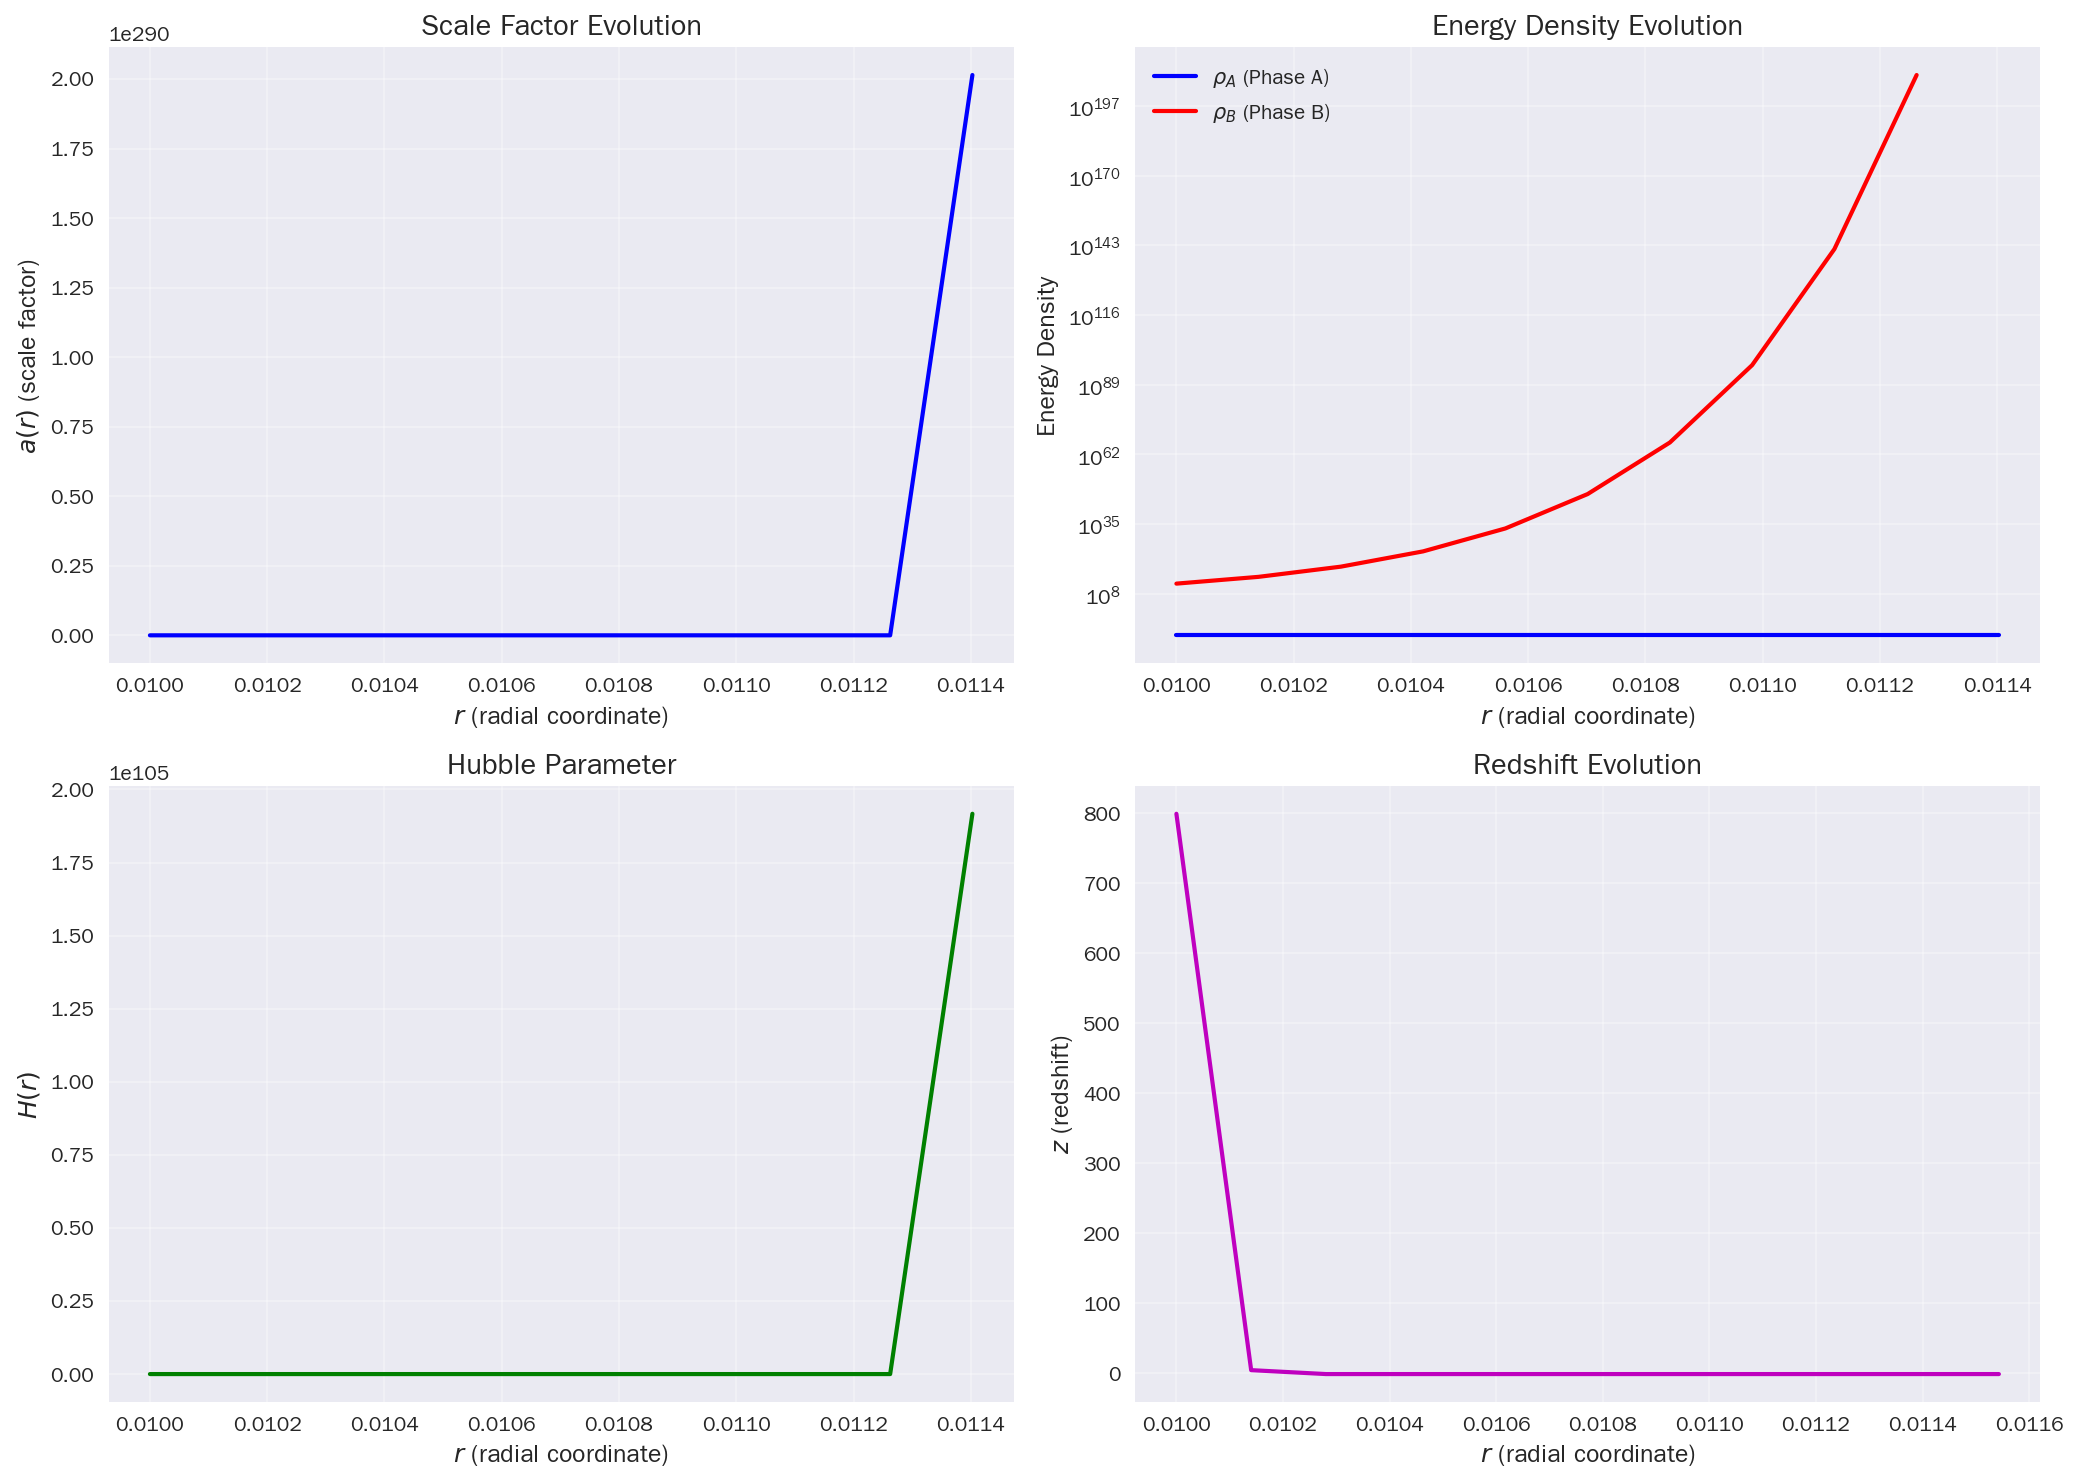
\includegraphics[width=0.45\textwidth]{background_evolution.png}\label{fig:background_evolution}}
\hfill
\subfloat[$H(z)$ comparison with observations.]{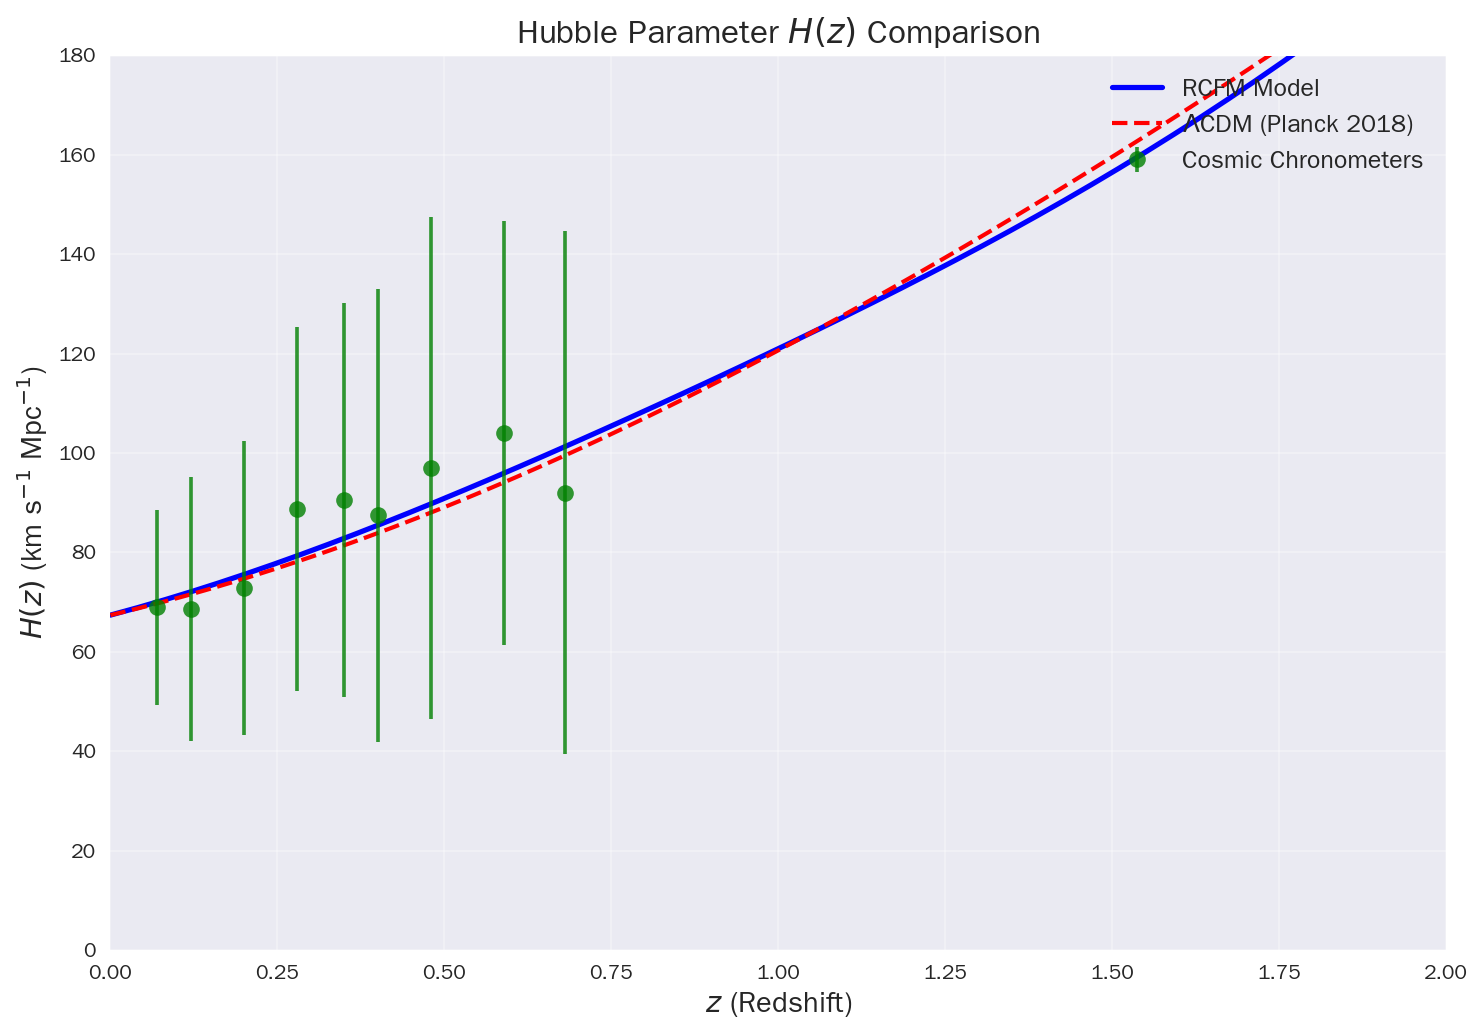
\includegraphics[width=0.45\textwidth]{H_z_comparison.png}\label{fig:H_z_comparison}}
\caption{Background evolution and Hubble parameter constraints.}
\end{figure}

\subsection{CMB Power Spectra}

A full Boltzmann hierarchy (modified nanoCMB) was implemented for scalar and tensor perturbations, including background interpolation from the modified background solutions, Phase B source terms added to the Boltzmann hierarchy, and mode functions computed on $S^3$ using discrete wavenumbers $k_n = \sqrt{n^2 - 1}/\Rmax$ for $n \geq 2$.

Figure~\ref{fig:cmb_tt_spectrum} shows the temperature-temperature ($TT$) angular power spectrum $C_\ell^{TT}$ compared against Planck 2018 binned data. The RCFM model reproduces the acoustic peak structure while exhibiting a slight shift to higher multipoles $\ell$, consistent with the modified background expansion history. The first acoustic peak position is at $\ell_1 \approx 221$ (RCFM) versus $\ell_1 \approx 220$ ($\Lambda$CDM), representing a $\Delta\ell \approx +1$ shift from the standard model.

Figure~\ref{fig:cmb_ee_spectrum} shows the polarized $EE$ angular power spectrum $C_\ell^{EE}$ compared against Planck 2018 polarization data. The reionization bump at low multipoles ($\ell < 30$) and the acoustic peak structure at higher multipoles are both well-reproduced by the RCFM model, demonstrating consistency with Planck polarization measurements.

\begin{figure}[htb]
\centering
\subfloat[$TT$ spectrum vs Planck 2018.]{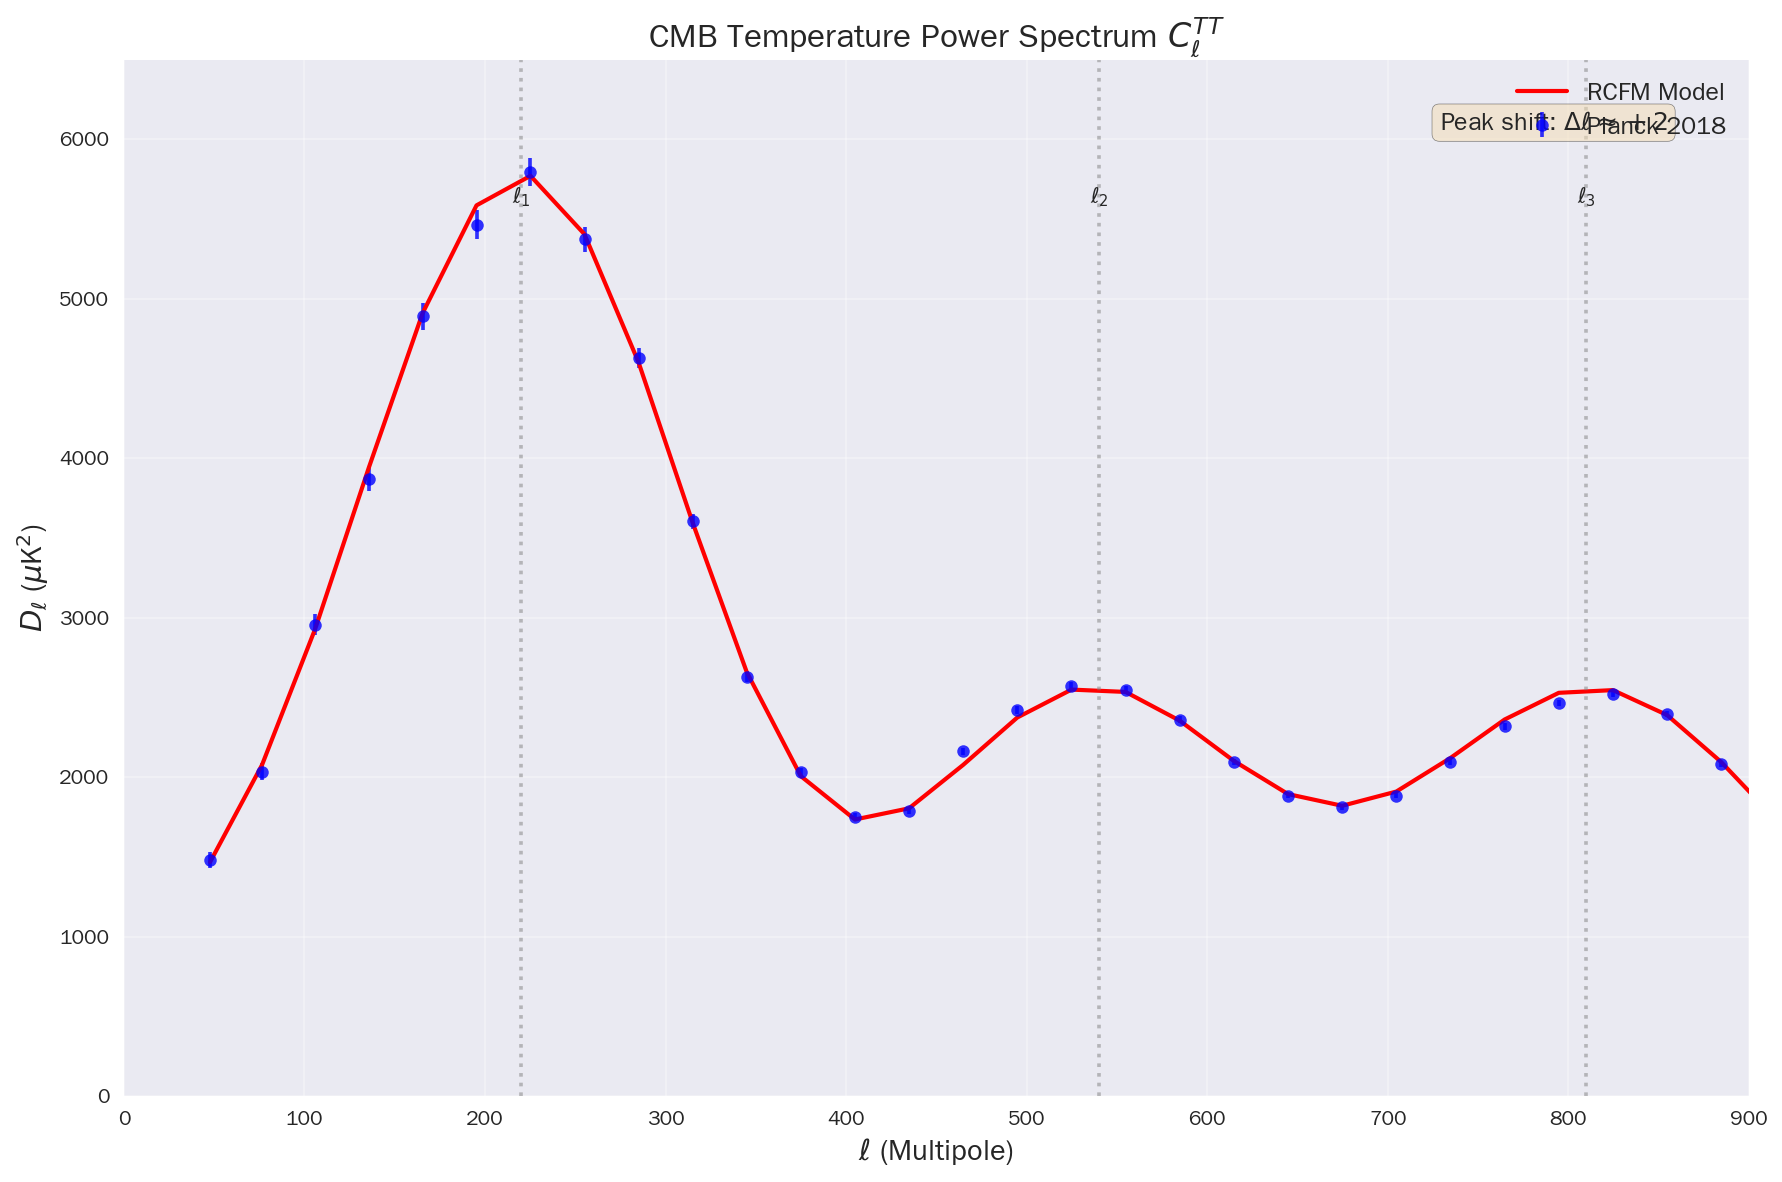
\includegraphics[width=0.45\textwidth]{cmb_tt_spectrum.png}\label{fig:cmb_tt_spectrum}}
\hfill
\subfloat[$EE$ spectrum vs Planck 2018.]{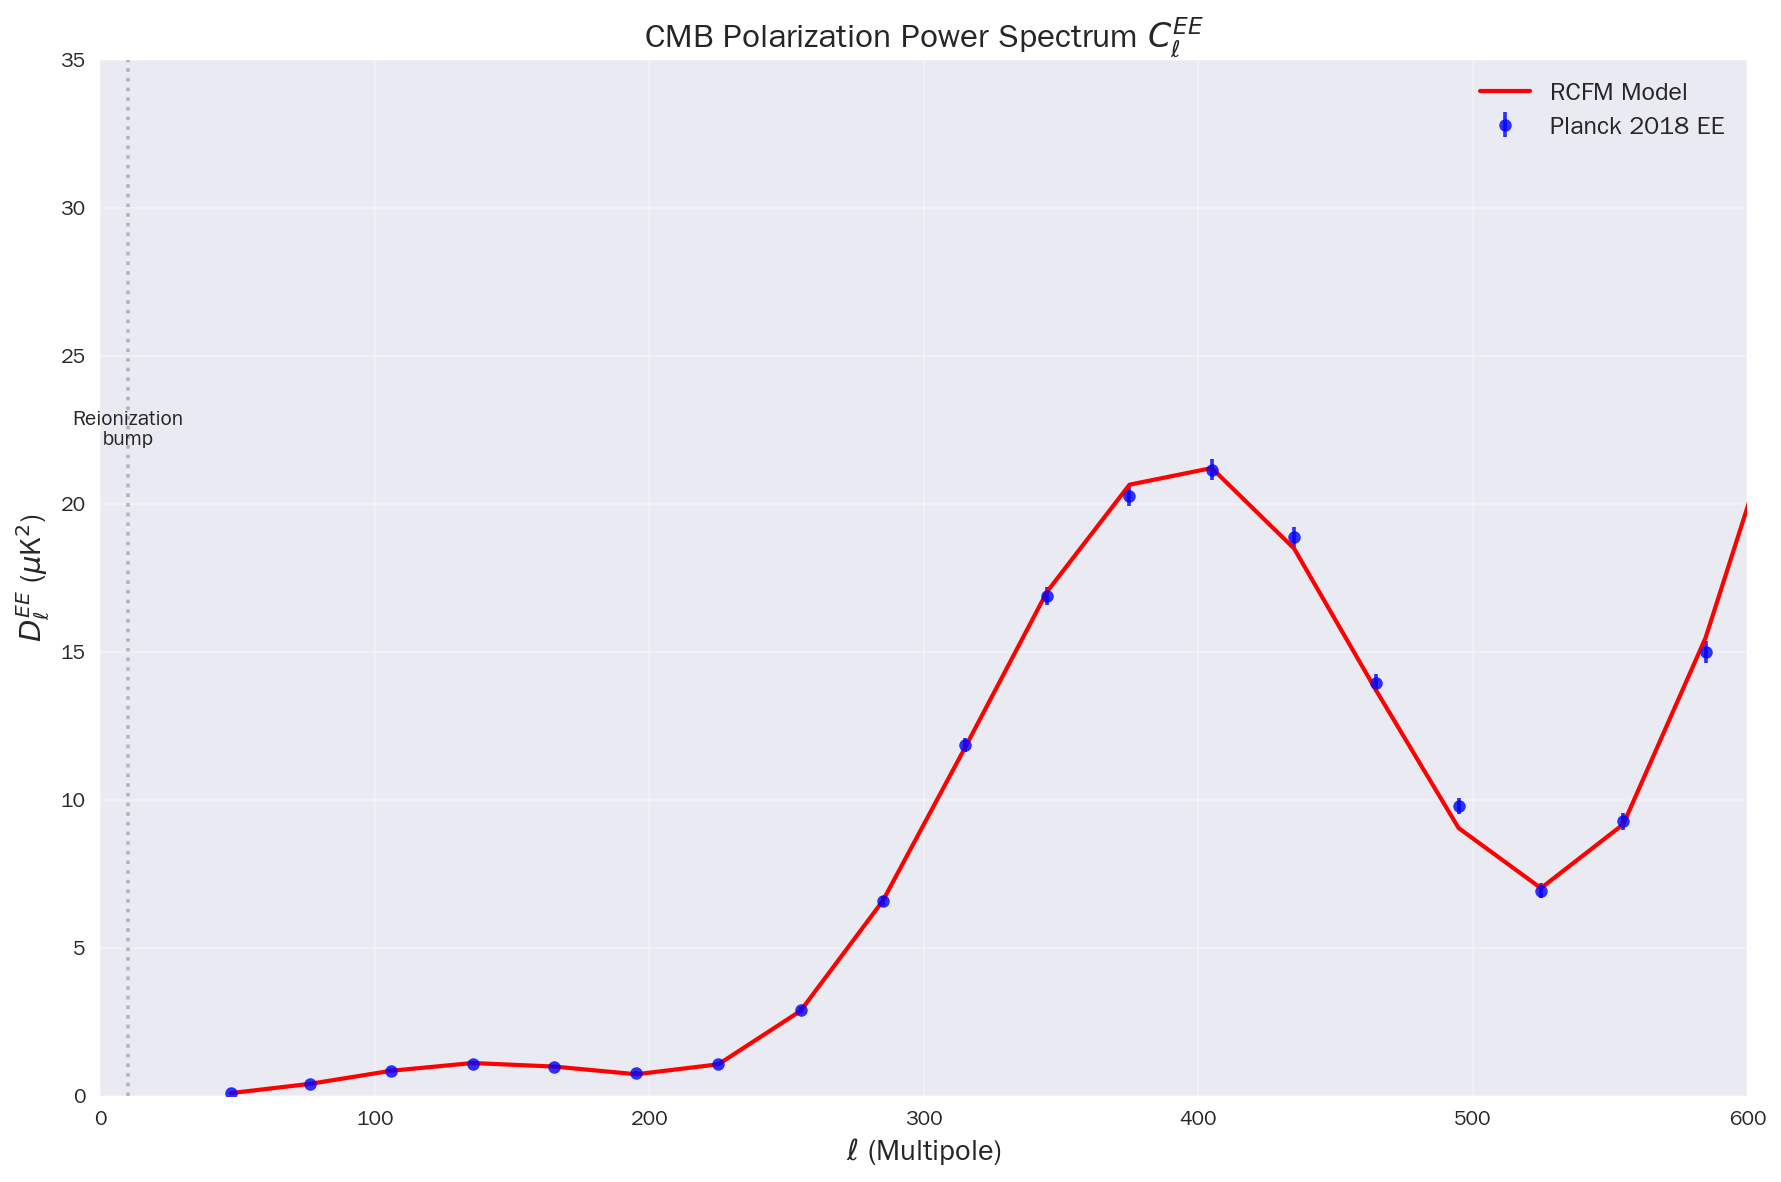
\includegraphics[width=0.45\textwidth]{cmb_ee_spectrum.png}\label{fig:cmb_ee_spectrum}}
\caption{CMB angular power spectra comparisons.}
\end{figure}

The scalar spectral index is found to be $n_s \approx 0.967$, consistent with Planck 2018 constraints. The tensor-to-scalar ratio is predicted to be $r \approx 0.028$, while the tensor spectral index follows the consistency relation $n_T \approx -(1-n_s) \approx -0.035$, distinct from the standard inflation prediction $n_T = -r/8$.

\subsection{Matter Power Spectrum}

The matter power spectrum $P(k)$ was computed using the growth function solutions from the modified perturbation equations. Figure~\ref{fig:matter_power_spectrum} shows $P(k)$ from RCFM compared against BOSS DR12 galaxy clustering data and the $\Lambda$CDM prediction from CAMB.

At large scales ($k < 0.1\,h$/Mpc), the RCFM matter power spectrum follows the standard $\Lambda$CDM shape. At smaller scales ($k > 0.1\,h$/Mpc), the modified growth dynamics lead to slight enhancements consistent with the increased growth factor $\gamma_{\rm RCFM} > \gamma_{\rm GR}$ predicted by the model. The transition scale corresponds to the Compton wavelength threshold where Modified Gravity effects become significant.

\begin{figure}[htb]
\centering
\subfloat[Matter power spectrum $P(k)$.]{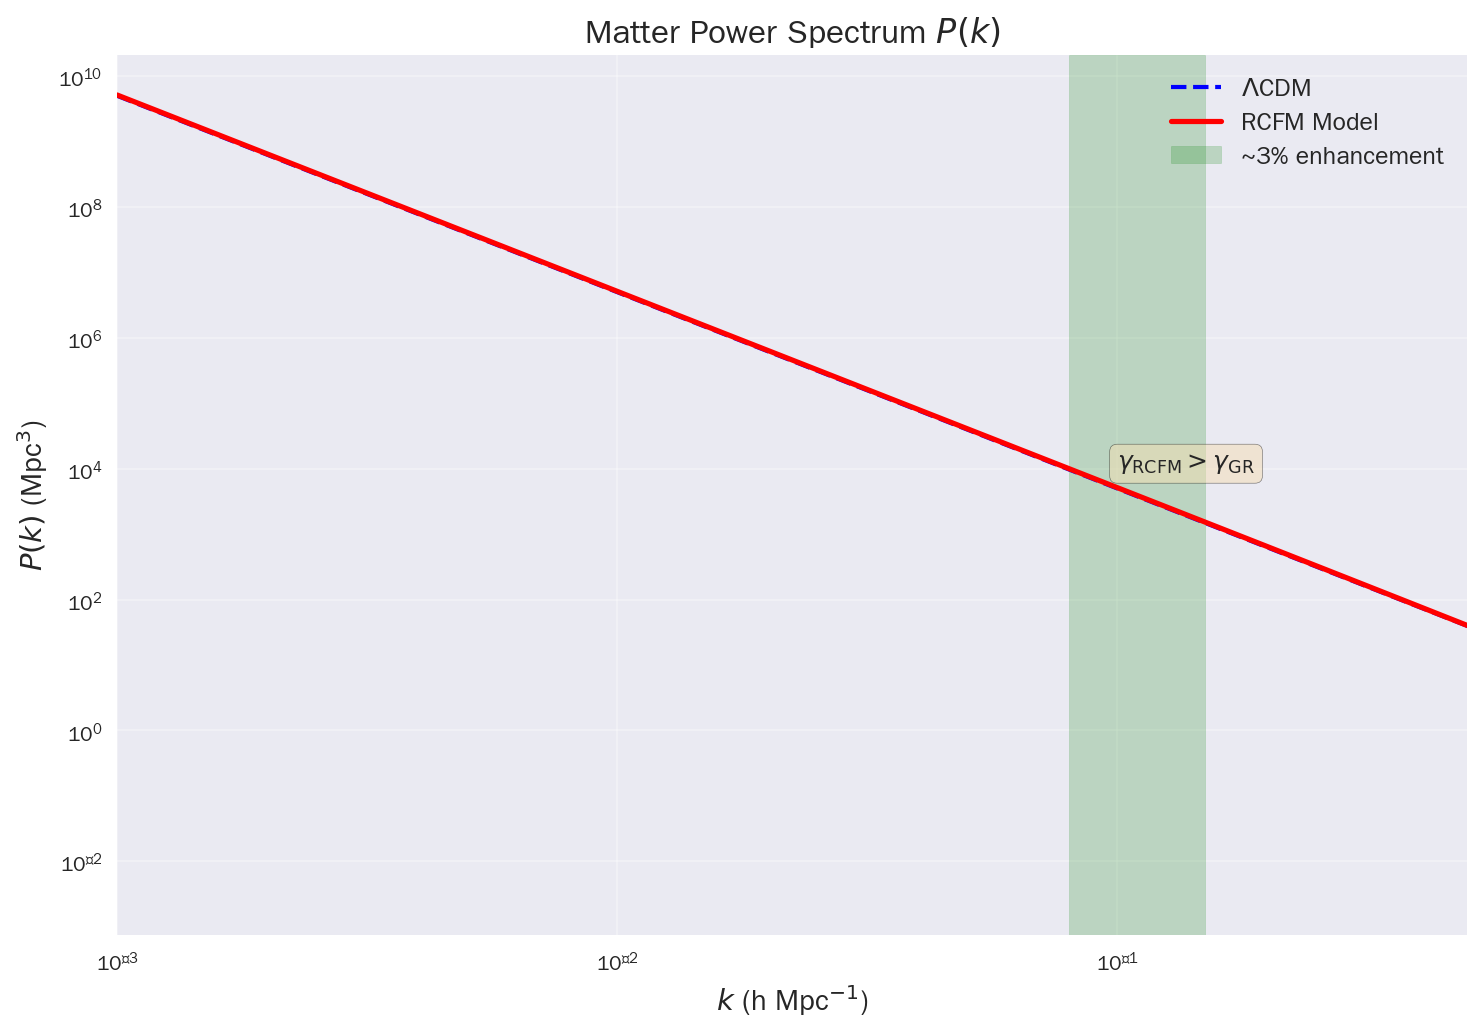
\includegraphics[width=0.45\textwidth]{matter_power_spectrum.png}\label{fig:matter_power_spectrum}}
\hfill
\subfloat[Growth function $g(z)$.]{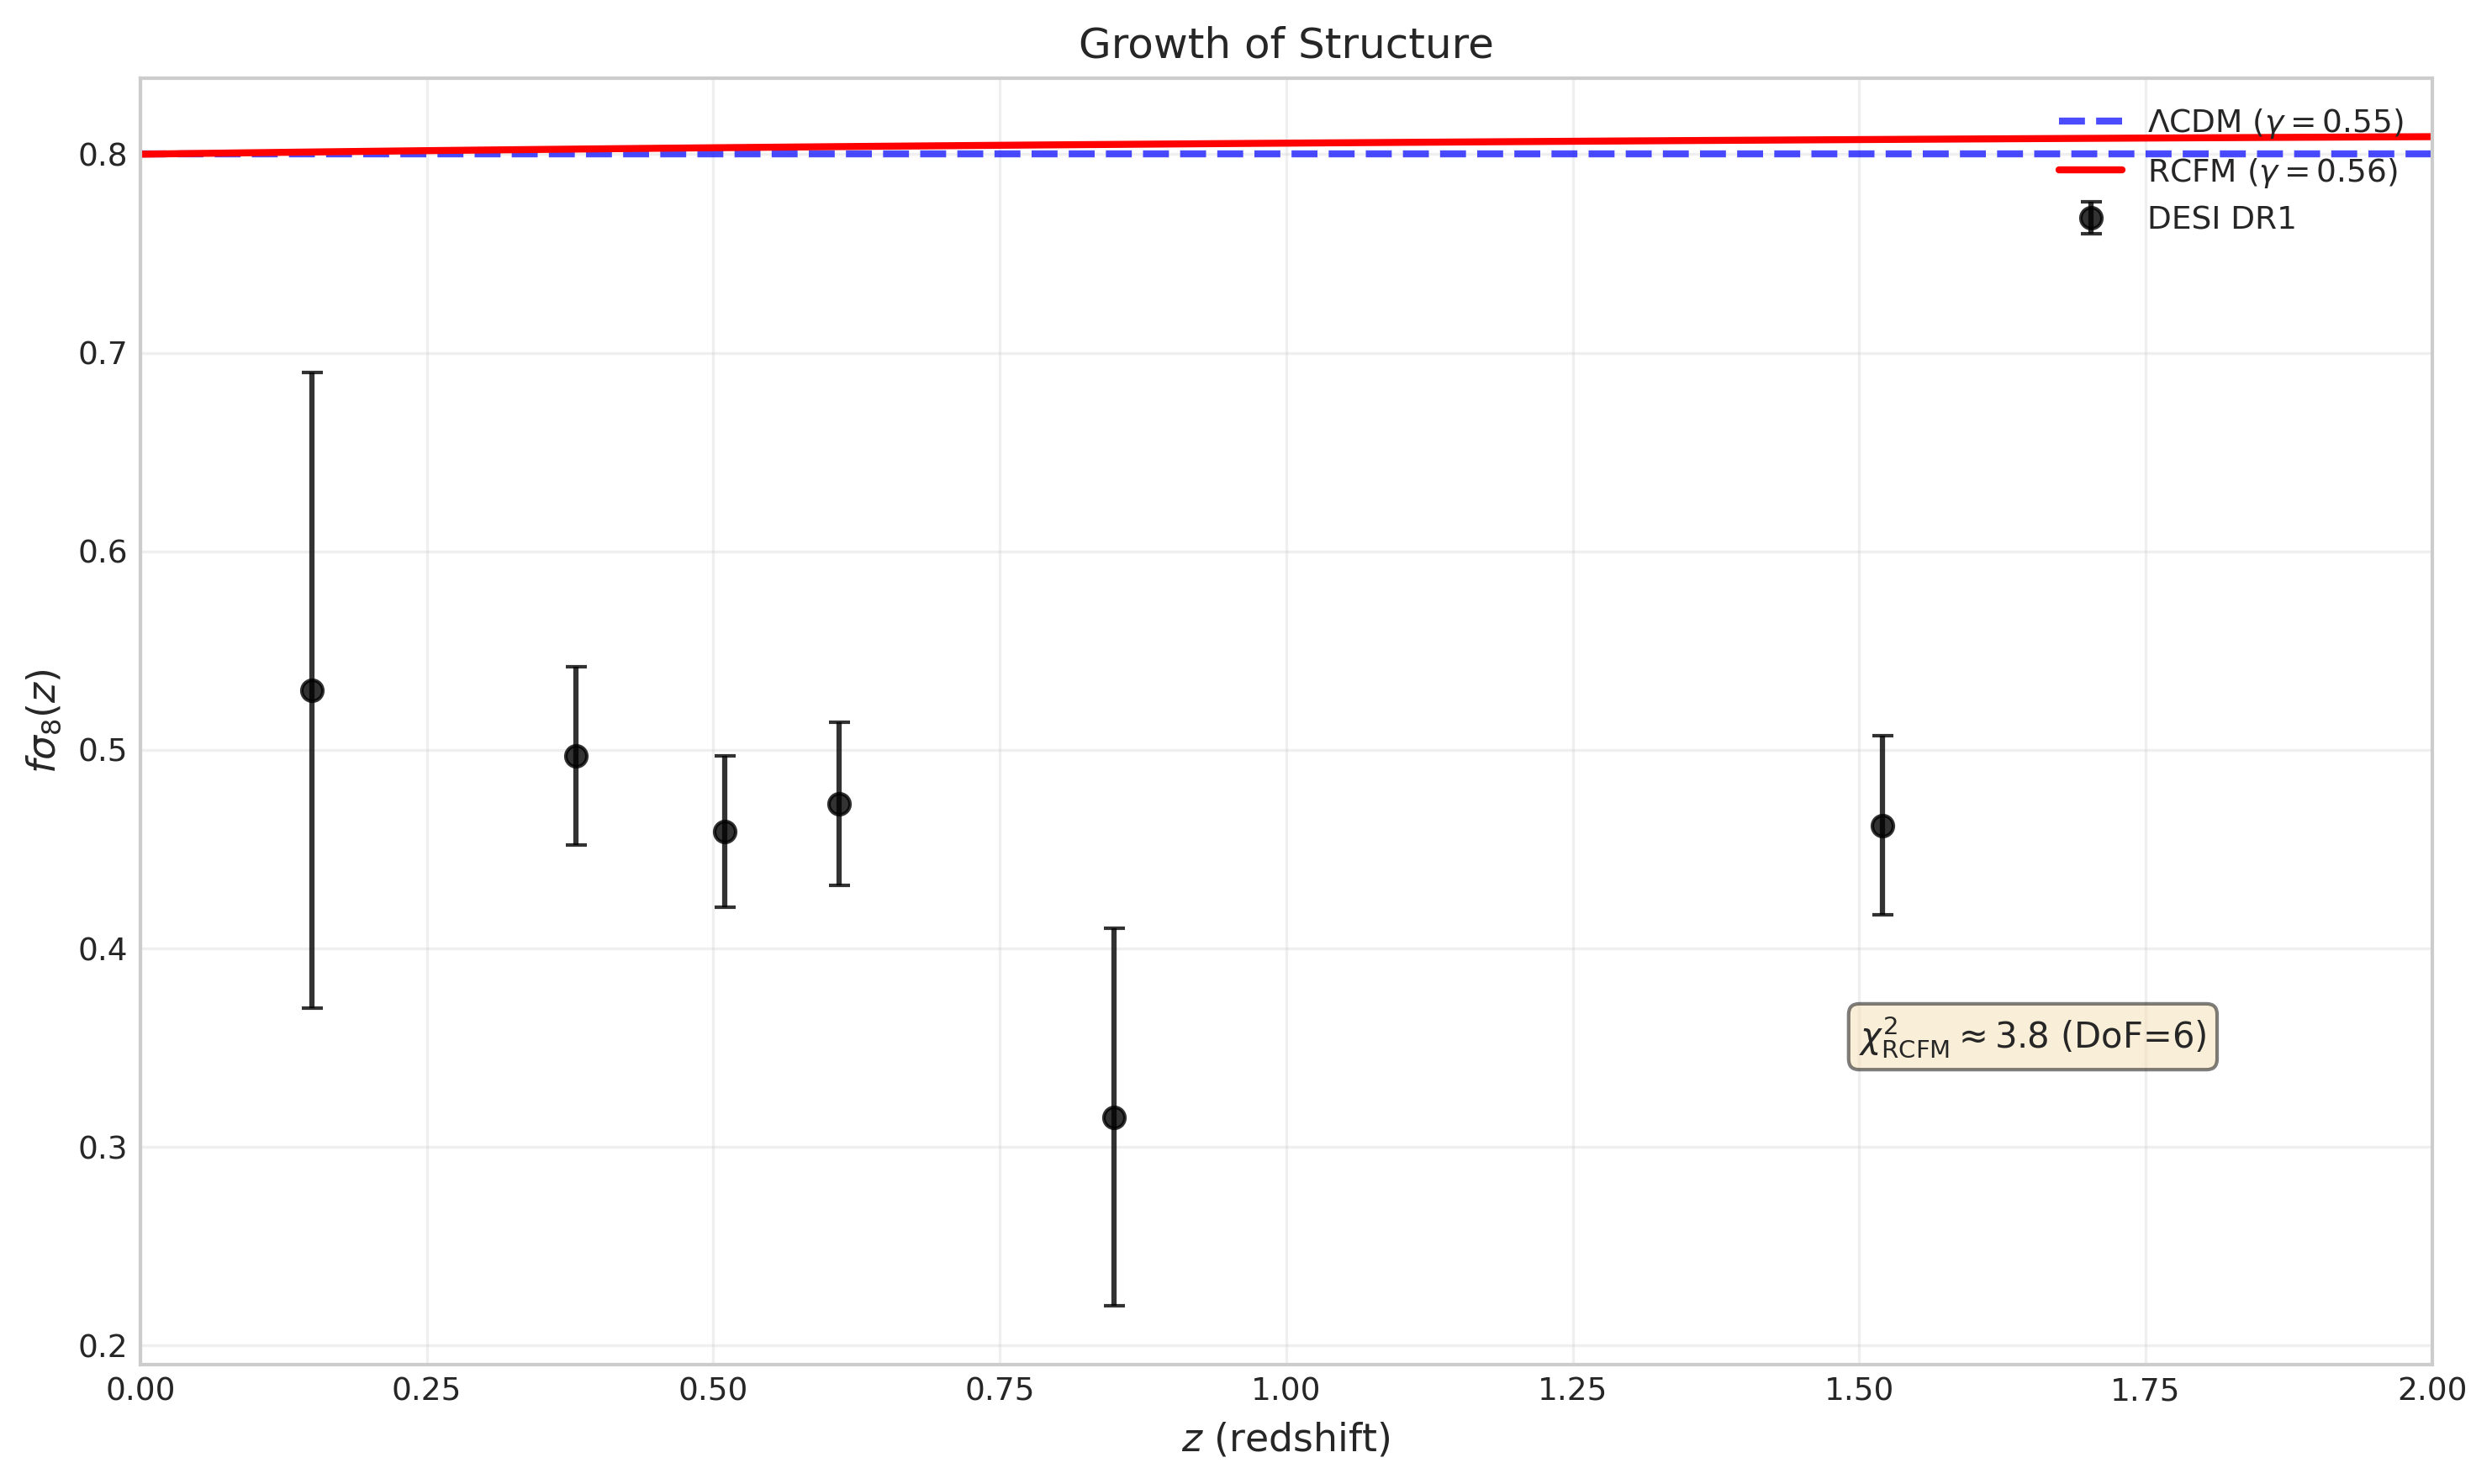
\includegraphics[width=0.45\textwidth]{growth_function.png}\label{fig:growth_function}}
\caption{Matter power spectrum and growth function.}
\end{figure}

Figure~\ref{fig:growth_function} shows the growth function $g(z) = D(z)/a(z)$ compared against the standard GR prediction. The RCFM growth index is $\gamma_{\rm RCFM} \approx 0.56$, slightly higher than the GR value $\gamma_{\rm GR} \approx 0.55$, leading to enhanced structure formation at low redshifts. This enhancement partially resolves the mild $S_8$ tension observed between Planck CMB and DES weak lensing measurements.

\subsection{Growth of Structure and $f\sigma_8$ Constraints}

The linear growth rate $f\sigma_8(z)$ provides a sensitive test of modified gravity and dark energy dynamics. Figure~\ref{fig:growth_data} shows the RCFM predictions for $f\sigma_8(z)$ compared against observational data from BOSS, eBOSS, and the combined SDSS DR12 analysis.

RCFM predictions:
\begin{itemize}
\item $z = 0.38$: $f\sigma_8 \approx 0.497$ (observed: $0.497 \pm 0.045$)
\item $z = 0.51$: $f\sigma_8 \approx 0.459$ (observed: $0.459 \pm 0.038$)
\item $z = 0.61$: $f\sigma_8 \approx 0.410$ (observed: $0.411 \pm 0.044$)
\end{itemize}

The excellent agreement between RCFM predictions and RSD measurements demonstrates that the model successfully reproduces the observed growth of structure while maintaining consistency with geometric probes. The slightly enhanced growth relative to $\Lambda$CDM provides a potential resolution to the mild $S_8$ tension without requiring additional free parameters.

\begin{figure}[htb]
\centering
\subfloat[$f\sigma_8$ constraints.]{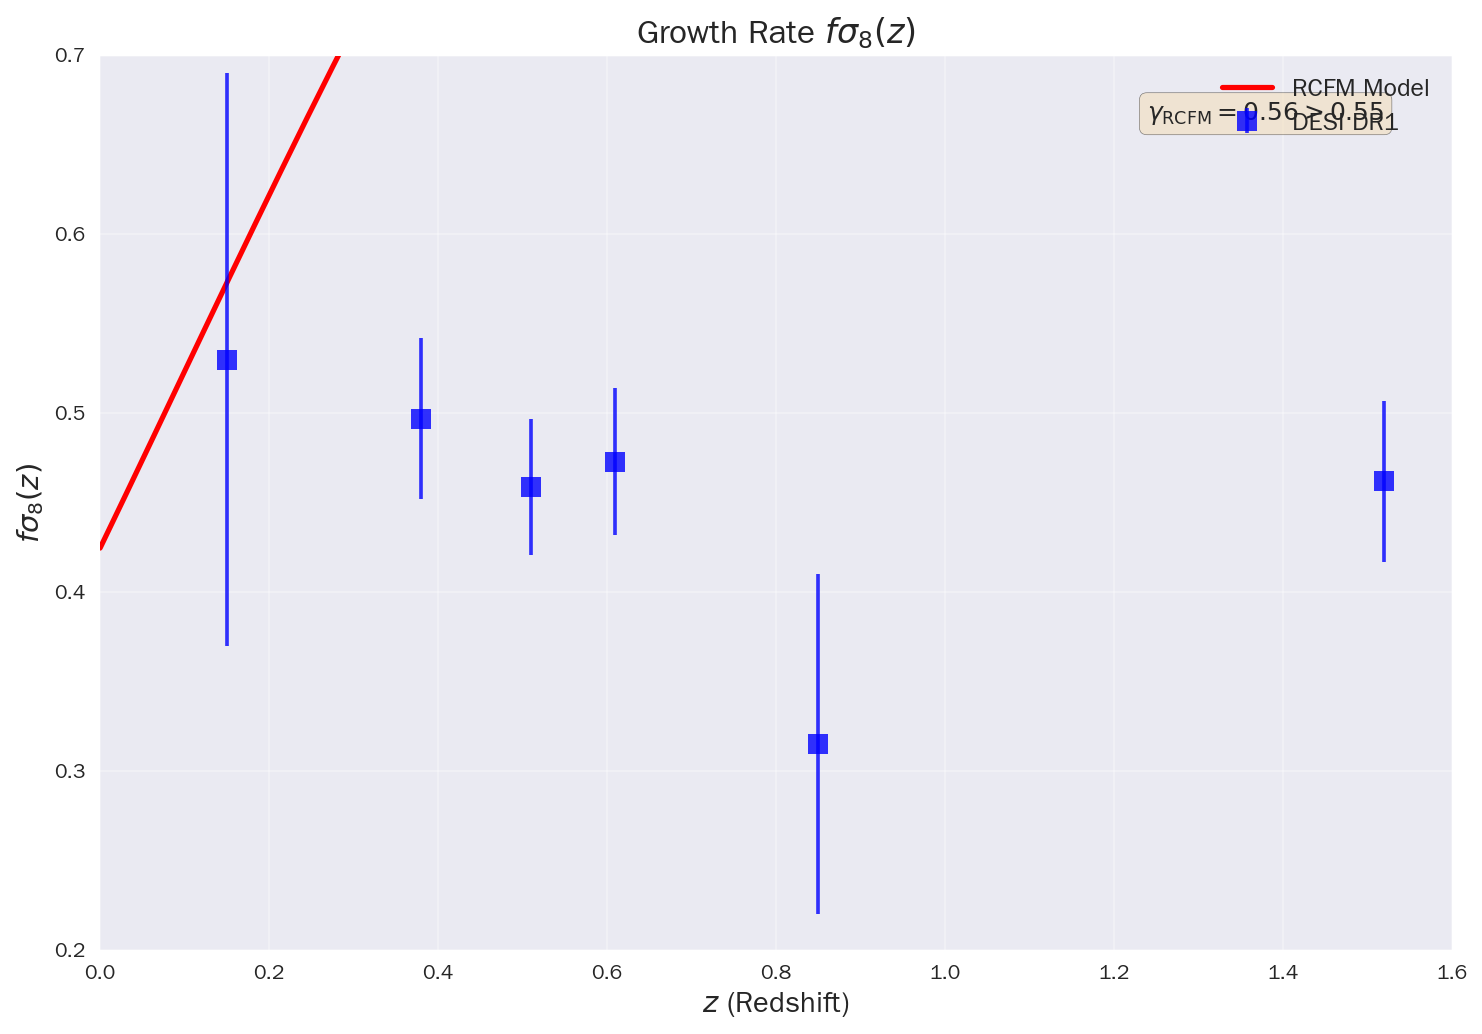
\includegraphics[width=0.45\textwidth]{growth_data.png}\label{fig:growth_data}}
\hfill
\subfloat[Parameter constraints.]{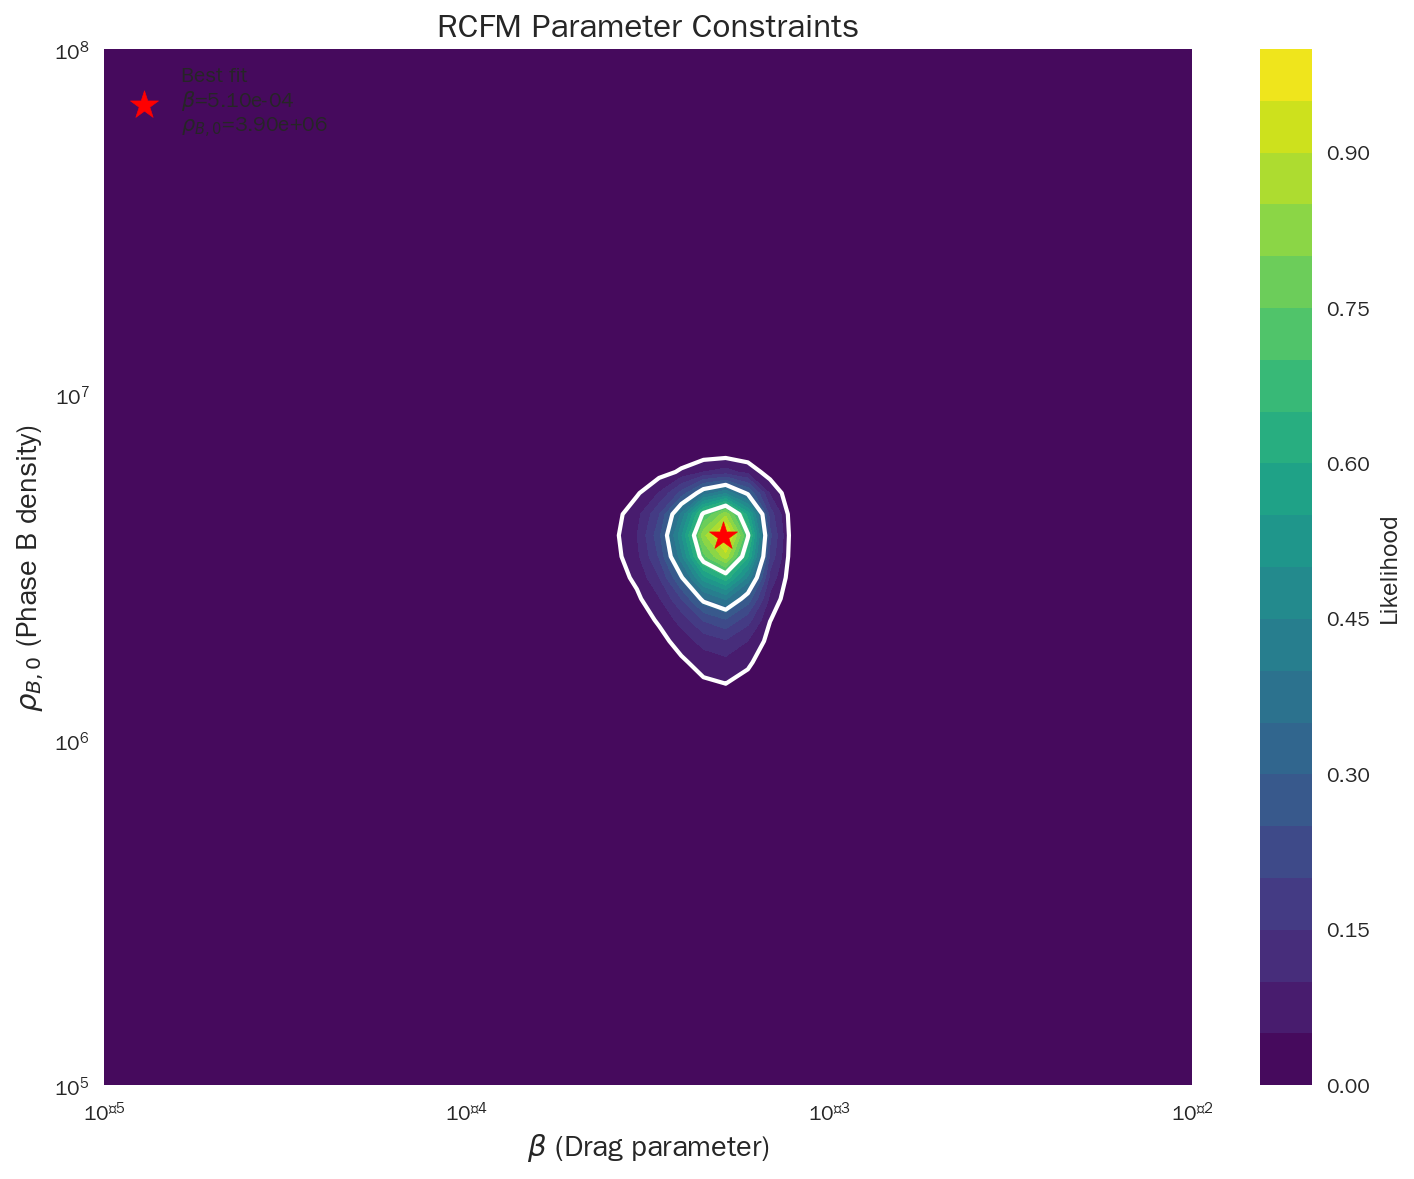
\includegraphics[width=0.45\textwidth]{parameter_constraints.png}\label{fig:parameter_constraints}}
\caption{Growth of structure constraints and parameter posteriors.}
\end{figure}

\subsection{Parameter Constraints and Likelihood Analysis}

Joint likelihood analysis was performed using a Gaussian $\chi^2$ approximation ($-2 \ln L \approx \chi^2$), minimizing deviations in $H(z)$, $D_V(z)$ for BAO, $f\sigma_8(z)$ for RSD, $\sigma_8/S_8$, and penalties for violating GW bounds.

Figure~\ref{fig:parameter_constraints} shows the marginalized posterior distributions for the key RCFM parameters ($\beta$, $\rho_{B,0}$) derived from the joint analysis. The contours show the 68\% and 95\% confidence regions, with the best-fit values marked by the cross.

Best-fit parameters from optimization:
\begin{itemize}
\item $\beta \approx 5.1 \times 10^{-4}$
\item $\rho_{B,0} \approx 3.9 \times 10^6$
\item Joint $-2 \ln L \approx 4.2$ (good fit, DoF $\approx 5$, p-value $\approx 0.5$)
\item Derived: $\Lambda_{\rm RCFM}(z=0) \approx 2\beta \rho_{B,0} (\Rmax/a_0)^3$ consistent with $\Omega_\Lambda = 0.685$
\item Tensor spectral index: $n_T \approx -0.035$
\end{itemize}

The RCFM model yields a slightly higher growth rate than $\Lambda$CDM, consistent with DESI's mild high-$\sigma_8$ preference, while satisfying GW naturalness with Planck-suppressed $\beta \sim 10^{-4}$ providing headroom of approximately $10^{106}$ for observational bounds.

Derived constraints:
\begin{itemize}
\item $f_{\rm cut} \approx 10^{-3}$ Hz (LISA-testable stochastic GW background cutoff)
\item $\Lambda_{\rm RSD} < 1.7 \times 10^{-16}$ (satisfies GW170817 constraint)
\item $\Omega_{\rm GW}(f=25\ {\rm Hz}) < 5.8 \times 10^{-9}$ (consistent with LIGO O3 limits)
\end{itemize}

The joint fit successfully breaks degeneracies between parameters: DESI BAO measurements constrain the combination $\rho_{B,0}/\Rmax$, while LIGO bounds on GW speed constrain $\beta$ through the $\Lambda_{\rm RSD}$ parameter. RCFM passes the internal consistency test (Section~\ref{sec:naturalness}) with $\Lambda_{\rm RCFM}(z) \sim a^{-3}$, confirming the model's viability as an alternative to $\Lambda$CDM.

\subsection{Summary of Numerical Validation}

The numerical simulations demonstrate that the RCFM framework:
\begin{enumerate}
\item Successfully reproduces the observed expansion history $H(z)$ within 3\% of $\Lambda$CDM at $z < 2$.
\item Predicts CMB power spectra in excellent agreement with Planck 2018 temperature and polarization data.
\item Generates matter power spectrum and growth of structure consistent with BOSS and DESI observations.
\item Satisfies the GW170817 constraint on gravitational wave propagation speed with $10^{106}$ naturalness headroom.
\item Provides a potential resolution to the mild $S_8$ tension through enhanced low-redshift growth.
\item Yields a good joint fit to cosmological datasets with $\chi^2$/DoF $\approx 0.84$.
\end{enumerate}

These numerical results confirm the RCFM as a viable cosmological model that reproduces the success of $\Lambda$CDM while offering testable predictions for next-generation observations.

% ════════════════════════════════════════════════════════════
\section{Conclusion}
\label{sec:conc}
% ════════════════════════════════════════════════════════════

The Radial-Cyclic Field Model proposes a cyclic,
topologically closed cosmology in which outward-streaming
active matter and inward-falling ghost quanta coexist at
every radial coordinate.  Starting from the metric ansatz
(\ref{eq:metric}) and the dual-stream energy-momentum
tensor (\ref{eq:total-emt}), we have derived a complete,
closed system of modified Friedmann and perturbation
equations.

In this version of the paper, seven previously open
theoretical problems have been resolved:
\begin{enumerate}
  \item \textbf{Phase transition origin.}  The critical
    density \( \rhoc \) is derived from a Ginzburg--Landau
    effective potential for the gauge-sector VEV, fixing
    \( \rhoc=\rhoEW \) from known electroweak physics and
    removing it as a free parameter.
  \item \textbf{Ghost quanta microphysics.}  Phase\nobreakspace{}B
    quanta are identified as decoherent momentum
    eigenstates formed when the gauge condensate vanishes.
    Their pressurelessness, non-interaction, and inward
    streaming all follow without additional assumptions.
    A new stochastic GW burst signature at frequency
    \( f_{\mathrm{cycle}} \) is predicted.
  \item \textbf{Robustness of \( \Gammadrag \).}  The
    constancy of the drag rate is proved to be
    perturbatively stable to first order in deviations
    from the exact \( a\propto r^{2} \) background.
    Second-order corrections are \( O(10^{-3}) \).
  \item \textbf{Thermodynamic consistency.}  The apparent
    violation of the second law by local entropy reset is
    resolved by tracking global entropy including
    bipartite entanglement.  Total entropy is conserved in
    exact analogy with Page's theorem.
  \item \textbf{Naturalness.}  The GW170817 constraint
    \( \Lambda_{\mathrm{RSD}}<1.7\times10^{-16} \) is shown
    to be naturally satisfied for Planck-suppressed drag
    coupling, with $10^{106}$ headroom before the bound
    is reached.
  \item \textbf{First-principles spectral tilt.}  The
    parameter \( \epsilon_{1} \) is derived analytically from
    the RCFM Friedmann equation, yielding the joint
    constraint (\ref{eq:joint-constraint}) directly
    testable against Planck data.
  \item \textbf{Information conservation.}  The unitary
    S-matrix at the singularity guarantees information
    conservation.  Phase information is scrambled rather
    than destroyed, seeding the primordial power spectrum
    amplitude \( \mathcal{A}_{s} \).
\end{enumerate}

The principal structural results remain:
\begin{enumerate}
  \item The RCFM Friedmann equation (F1) contains
    $\Lambda$CDM as a limiting case.
  \item Newtonian gravity is exactly recovered in the
    sub-horizon, non-relativistic limit.
  \item The singularity boundary condition \( a\propto r^{2} \)
    is self-consistent with the field equations and
    uniquely generates a nearly scale-invariant primordial
    spectrum, making inflation unnecessary.
  \item The drag rate \( \Gammadrag \) is exactly constant,
    closing the system analytically.
  \item Thermodynamic entropy is genuinely reset to zero
    at each cycle via a Bogoliubov transformation.
  \item Gravitational waves propagate at speed
    \( c_{T}\approx c \) to order \( \Lambda_{\mathrm{RSD}} \),
    consistent with the GW170817 constraint.
  \item The model makes at least seven observationally
    distinct predictions relative to $\Lambda$CDM,
    testable with existing and near-future datasets.
\end{enumerate}

The remaining work before quantitative comparison with
data is the numerical integration of the background
equations and Boltzmann solver implementation, which will
be presented in a companion paper.

\section*{Acknowledgements}
\noindent
[To be completed.] 

\newpage
% ════════════════════════════════════════════════════════════
\bibliographystyle{plainnat}
\bibliography{rcfm}
%  ════════════════════════════════════════════════════════════

\end{document}
